\section{Introduction} \label{sec:introduction}

Energy efficiency has been one of the main focuses in computing nowadays, both on mobile and HPC. It is essential to increase battery life and reduce heat generation, especially in high-performance computing (HPC), where a small percentage of the savings energy can significantly reduce maintenance costs or environmental impact due to its scale of consumption. For example, the leading Petaflop supercomputers consume in the range of 1 to 18 MW of electrical energy, with 1.5 MW on average, which we can estimate in millions of dollars in annual electricity cost \cite{Group2012HandbookSahni}. Furthermore, the International Energy Agency \cite{iea_2021} estimated that global data center electricity usage in 2020 was around 200-250 TWh, or around 1\% \cite{Corcoran2017EmergingICT} of global electricity demand, which could generate as much pollution as a nation like Argentina \cite{Mathew2012Energy-awareNetworks}.

Given the importance of this topic, modern desktops, cell phones, and HPC CPUs have built-in power management mechanisms. That is because the processor is one of the main components that drain energy and can reach 50\% of the total system consumption \cite{Fan2007, Barroso2007TheComputing, Malladi2012TowardsDRAM}. Among the mechanisms implemented by the CPU, the most impactful and controllable via software are Dynamic Frequency and Voltage Scaling (DVFS), and Dynamic Power Management (DPM) ~\cite{Rotem2012Power-managementBridge, Brown2005, Hackenberg2015}.

DPM encompasses a set of techniques that take advantage of different energy levels in the system, such as active, inactive, and disabled~\cite{CARDOSO201717, Shuja2012Energy-efficientCenters, Benini2000AManagement}. The basic idea is to turn off devices and turn them on when needed. However, it is not a trivial task, and several variables need to be considered, such as the cost of switching, in terms of time and energy, how long it will remain in that state, the energy consumption in each state, and much more.

The DPM technique has the most significant gains when in systems where the static power is very high or where the system is idle for a long time. In such cases, some papers report savings of up to 70\% in energy~\cite{Shuja2012Energy-efficientCenters, Benini2000AManagement}.

DVFS, on the other hand, allows real-time frequency and voltage control, depending on needs. This method is motivated by the fact that we can approximate the relationship of frequency to power as a cubic equation and frequency and performance as a linear equation \cite{Dayarathna2016DataSurvey, Group2012HandbookSahni} implying that a reduction in frequency has a cubic impact on power and linear performance. Still, it is not so simple because lowering the frequency leads to longer runtime, increasing power consumption. As a result, determining the best voltage and frequency to employ under all conditions is also a challenging task.

Although there are many studies on this topic, most works focus on implementing different optimization algorithms based on workload, and few studies pay attention to phase division. Instead, most studies use static phase division to simplify the optimization math and compensate by implementing lightweight algorithms. However, this leads to a sub-optimization, as another phase division could result in different frequency values. In addition, there is an overhead associated with the moment the algorithm takes action that could be reduced if we knew the ideal moment for it to take action, making it possible even to allow heavier algorithms. Therefore, this work proposes a methodology to study the division of time (phases) and analyzing possible gains.

\section{Related work} \label{sec:related_work}

One of the bases works in scheduling algorithms is the work of Irani et al. \cite{Irani2007}, where they formalized the problem of scheduling arriving jobs in a way that minimizes total energy use and so that each job is completed after its arrival time and before its deadline. Although each problem has been considered separately, this was the first theoretical analysis of systems that can use both mechanisms.

Past work has also used feedback-based approaches, as in Poellabauer et al. \cite{Poellabauer2005}, where applications' past CPU utilization's are used to predict future  CPU  requirements. However, mispredictions in these approaches can lead to missed deadlines,  sub-optimal energy savings,  or large overheads due to frequent changes to the chosen frequency or voltage. One shortcoming of previous approaches is that they ignore other 'indicators' of future CPU requirements, such as the frequency of I/O operations, memory accesses, or interrupts.

In the thesis work of Saha et al. \cite{Saha2012}, the timeliness and power consumption behavior of fourteen RT-DVFS schedulers through implementation and actual measurements. The schedulers include Static Earliest Deadline First (Static-EDF), Cycle Conserving Earliest Deadline First(CC-EDF), Look-Ahead Earliest Deadline First (LA-EDF), Snowdon-minimum (Snowdon-min), Resource-constrained Energy-Efficient Utility Accrual Algorithm (REUA), DynamicReclaiming Algorithm (DRA) and Aggressive Speed Reduction Algorithm(AGR) among the others. They draw attention to the fact that most of these algorithms are based on simulations, which can mislead some results. Broadly, RT-DVFS techniques have two objectives: (i) Reduce energy consumption through DVFS; and (ii) Optimize task timeliness behavior through real-time resource management (deadline).

Pietri et al. \cite{Pietri2014} used slack reclamation to achieve energy savings. The goal is to exploit the idle slots of the processors that occurred due to the earlier completion time of the tasks compared with the latest finish time, which is constrained by the deadline or data dependencies. In their model, the user submits a workflow for execution specifying a deadline for completion of the execution.

Mashayekhy et al. \cite{Mashayekhy2014} proposed a greedy algorithm, called Energy-aware  MapReduce  Scheduling  Algorithm  (EMRSA), that finds the assignments of the map and reduces tasks to the machine slots in order to minimize the energy consumed when executing the application. They consider an extensive data application consisting of a set of map and reduce tasks that need to be completed by deadline D.

Yousefi et al. \cite{Yousefi2018}  present a task-based greedy scheduling algorithm, TGSAVE. This algorithm selects a slot for each task to minimize the total energy consumption of the MapReduce job for big data applications in heterogeneous environments without significant performance loss while satisfying the service level agreement (SLA). TGSAVE  finds solutions under deadlines up to 74\% tighter than the tightest one feasible by EMRSA, and it can meet deadlines as tight as only12\%, on average, more significant than the energy-oblivious minimum makespan.

Crown scheduling is a static scheduling approach for sets of parallelizable tasks with a common deadline. Crown schedules are robust, i.e., the runtime prolongation of one task by a moderate percentage does not cause a deadline transgression by the same fraction. In addition, by speeding up some tasks scheduled after the lengthy task, the deadline can still be met at moderate additional energy consumption. In the work of Kessler et al. \cite{Kessler2021} they present a heuristic to perform this re-scaling online and explore the trade-off between additional energy consumption in normal execution and limitation of deadline transgression in delay cases.

%Typically target traditional real-time systems with static deadlines, resulting in conservative energy savings that cannot exploit additional energy optimizations due to dynamic deadlines. However, in the work of Yi et al. \cite{Yi2021} they present an adaptive system optimization and reconfiguration approach that dynamically adapts the scheduling parameters and processor speeds to satisfy dynamic deadlines while consuming as little energy as possible. As their work was for autonomous driving, they used velocities as deadlines.

In the work of \cite{Ajmal2021}, a green cloud computing algorithm named "Cost-based Energy Efficient Scheduling Technique for Dynamic Voltage Frequency Scaling (DVFS) Systems (CEEST)" is proposed. The proposed algorithm reduces energy consumption without compromising the quality of service (QoS). This algorithm aims to optimize and manage servers in the datacenters by utilizing maximum resources and powering off the underutilized servers. Furthermore, CEEST utilizes the scaling of virtual machines to finish jobs within the deadlines to reduce violations of service level agreement (SLA). 

All of these works at some point considered a deadline (defined by the user of the system) that defines the phases of the job; this means that choosing a different deadline could result in completed different energy savings, and because this is not the main focus of these works, this is not considered. In our paper, we study the impact of this phase division on the application's energy consumption. We estimate how much energy could be saved if an algorithm could magically give the ideal deadline.

Although most of the work is considered a deadline, some works include job division as part of the optimization problem. For example, in the paper of Agrawal et al. \cite{Agrawal2021}, they show that if the jobs can be divided into arbitrary parts, the minimum-energy schedule can be generated in linear time, giving exact scheduling algorithms. For the cases where jobs are non-divisible, they claimed a prove that the scheduling problems are NP-hard and also give approximation algorithms for the same along with their bounds. 

In this case, where no deadline is defined, the phase division is indirectly considered by solving the optimization problem of minimizing the energy. The problem, in this case, is that several constraints restrict the optimization problem while our approach works with measured data, meaning that we can find solutions independent of the constraints.

\section{Phase division approach} \label{sec:application_partition_method}
To find the optimal phase division, we would have to ensure that the one we choose is the most energy-efficient among all possible divisions and different combinations of power configurations.

This mathematical problem can be modeled in many ways, but always with some concessions to make it solvable. Another option would be by brute force, but there are infinite possibilities for splitting phases, although some hardware limitations make our analysis more accessible.

With that in mind, we decided to create a heuristic that comes the closest to brute force using hardware limitations to make it viable.

The first limitation is that the processor has a limited speed at which it can act. In other words, a division that can act would make no sense, limiting our analysis to discrete-time intervals at the processor's maximum performance speed.

This already limits our exploration space a lot, but even so, it is still unfeasible. For example, considering $d_t$ as the minimum processor action interval, $T$ the total application time, and $C$ the number of power settings. The number of possibilities could be estimated by:
\begin{equation}
	\left(\frac{T}{d_t}\right)^C,
\end{equation}
This number grows astronomically because $d_t$ is in a time range of microseconds, $T$ seconds or minutes, and C of hundreds. To give an idea, we can estimate this number to be in a range of $10^7000$.

Another thing that we can see is that each configuration gives the power profile for a given application, and phase division is just a combination of these configurations. This allows us to reduce further our exploration of space. For example, if we ran each power setting once and we had a way of combining them, our problem now would be feasible.

To make this possible, we assume that the configuration change only affects the program speed and that the power consumption is independent of the previous settings.

\iffalse %%%%%%%%%%%%%%%%%%%%%%%%%%%%%%%%%%%%%%%%%%%%%%% commented 
This means that in a certain part of the program $x_1$\% to $x_2$\% it will always execute the same instructions and the energy consumption would depend only on the configuration.

That said, if we treat the program as a percentage of execution, and we have the power consumption profile for all configurations, we can estimate the power consumption for any combination of phases.

For example if we have the phase division, 0-x_1\%, x_1\%-100\%, with the settings c_1 and c_2, the estimated energy would be:
P_{c_1}*u(0,x_1)*T_{c_1}+P_{c_2}*u(x_1, 100)*T_{c_2}

We can see that we just need a power profile P and the total runtime for each configuration and that we can divide the application into as many phases as we want.

For that we are going to assume that the number of instructions to complete a program is roughly the same independent on the frequency, thus we can write the number of instructions as:
\begin{equation}
	I=c_{k1}f_1T_1=c_{k2}f_2T_2,
\end{equation}
where $I$ is the number of instructions, $c_{k1}$ the rate of instructions per cycle, $f$ the frequency of the processor and $T$ the execution time. All the required parameters can be collected by simply running the application with the available frequencies. 

From this equation we can split the execution of the program into several different phases $i$ as follows:
% \begin{equation}
%     I=xI+(1-x)I=xc_{k1}f_1+(1-x)c_{k2}f_2
% \end{equation}
\begin{equation}
	I=\sum_{i}{a_iI} %=\sum_i{a_ic_{ki}f_i}
\end{equation}

with $a_i$ as the percentages of instructions executed with frequency $f_i$, we can compute any combination of phases. For convenience, we write this as a function of the time:
% \begin{equation}
% T=\frac{I}{c_{k1}f_1}
% \end{equation}
\begin{equation}
	I=Tc_{k}f
\end{equation}
\begin{equation}
	I=\sum_{i}{a_iI}=\sum_i{a_iTc_{ki}f_i}
\end{equation}
% \begin{equation}
% I=xI+(1-x)I=xTc_{k1}f_1+(1-x)Tc_{k2}f_2
% \end{equation}

the application being divided into phases of different duration, $a_i$  becomes the duration of the phase as a percentage of the total execution time. This general equation does not limit the number and duration of phases, and several phases can have the same frequency. 

In the event that we decide to include the number of cores as a context parameter, the equation becomes more complex. Indeed, the number of cores can completely change the application's behavior but, depending on the type of application, it's still possible to find similarities. Many HPC applications use data parallelism, and the Amdahl's law can model most of it. For this kind of applications, we can estimate that:
\begin{equation}
	T=\frac{T_s}{S}
\end{equation}
\begin{equation}
	T_s=\frac{I}{c_kf}
\end{equation}
\begin{equation}
	S=\frac{1}{1-w+\frac{w}{p}}
\end{equation}
\begin{equation}
	T=\frac{I(1-w+\frac{w}{p})}{c_kf}=\frac{I}{c_kf}-\frac{Iw}{c_kf}+\frac{Iw}{c_kfp}
\end{equation}

Looking at a fixed frequency, we arrive at a very similar structure as before:
\begin{equation}
	T=c_1I+\frac{c_2I}{p}
\end{equation}

As previously, we can use $I$ as the number of reference instructions, and compute $a$ as the percentage of single and multi-core instructions, or express it as a percentage of the total time T:
\begin{equation}
	aT=c_1aI+\frac{c_2aI}{p}
\end{equation}

The extent of the hypotheses will later be validated, however, by taking advantage of both principles, we can now, based on real measurements, estimate any phase division and possible context combination.
\fi %%%%%%%%%%%%%%%%%%%%%%%%%%%%%%%%%%%%%%%%%%%%%%%

This approach aims to bring the best of both worlds. We want simulation speed but with actual measurement data for greater accuracy. Our algorithm runs with measured data from a real system. The idea is to run the application with all possible configurations (e.g., frequency and number of active cores) of the machine without time division and estimate power consumption for different phase divisions.


\section{Building applications power profile} \label{sec:building_a_database}

%\subsection{Case-Study Architecture} \label{subsec:casestudyarchitecture}
%We executed the experiments in a system equipped with two Intel Xeon E5-2698 v3 processors with sixteen cores and two hardware threads for each core, with a total physical memory of the node is 128GB (8$\times$16GB). We disabled turbo frequency and hardware multi-threading during all experiments. The operating system used was Linux CentOS 6.5 and kernel 4.16. The overall view of the architecture is shown in \cref{fig:architecture}.
%
%\begin{figure}[H]
%	\centering
%	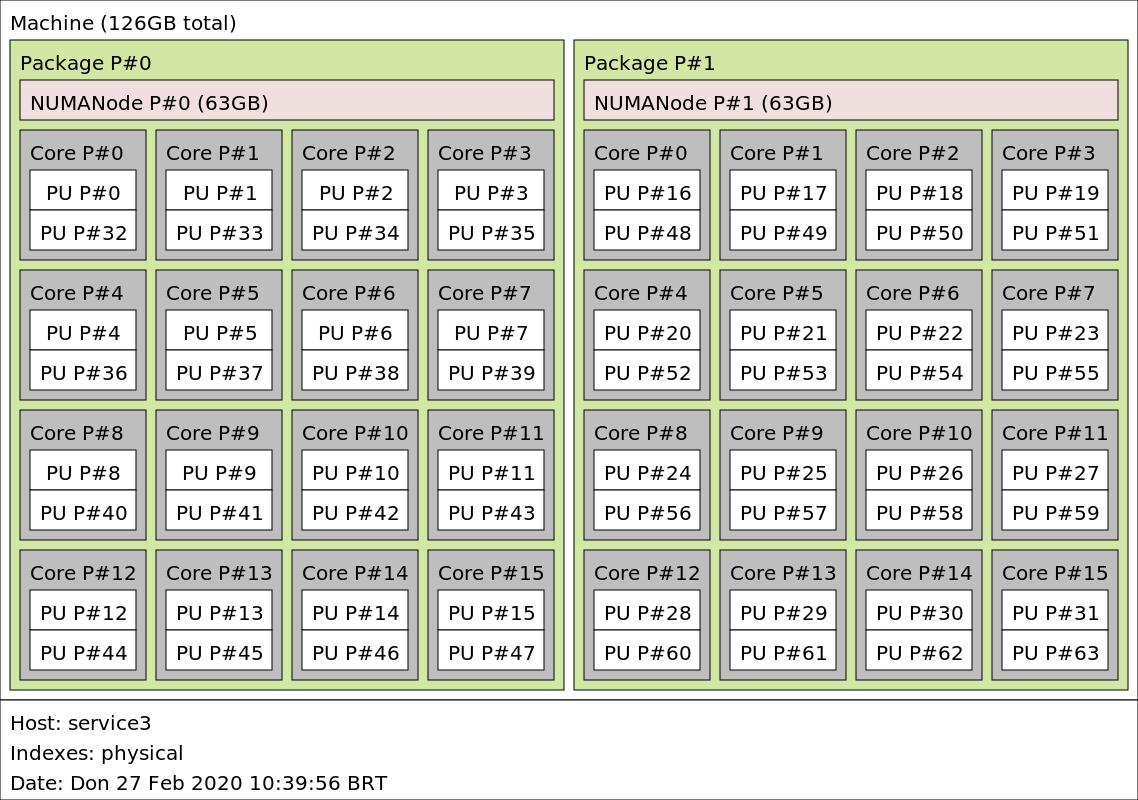
\includegraphics[width=0.8\columnwidth]{models/figures/architecture.png}
%	\caption{Node architecture (the image was made with the lstop application).}
%	\label{fig:architecture}
%\end{figure}
%
%To perform the frequency control, we used the acpi-cpufreq driver using the Userspace governor, which allows the user or any userspace program to set the CPU to a specific frequency. While the cores control was accomplished by modifying the appropriate system files with the default CPU-hotplug driver.
%
%The architecture is also equipped with the Intelligent Platform Management Interface (IPMI), a set of interfaces allowing out-of-band management of computer systems and platform-status monitoring via the local network~\cite{Schwenkler2006IntelligentInterface}. In addition, it can monitor variables and resources such as the system's temperature, voltage, fans, and power supplies, with independent sensors attached to the hardware.
%
%\subsection{Case-Study Applications} \label{subsec:casestudyapplication}
%The applications Black-Scholes, Bodytrack, Canneal, Dedup, Fluidanimate, Freqmine, Raytrace, Swaptions, Vips and x264 from the PARSEC \footnote{\url{https://parsec.cs.princeton.edu/download.htm}} parallel benchmark suite, version 3.0~\cite{Bienia2008TheSuite}, OpenMC \cite{Romano2015OpenMC:Development} and LINPACK (HPL) \cite{Dongarra1988TheExplanation}, were chosen as case studies. The PARSEC benchmark focused on emerging workloads and was designed to represent the next-generation shared-memory programs for chip-multiprocessors. It covers many areas such as financial analysis, computer vision, engineering, enterprise storage, animation, similarity search, data mining, machine learning, and media processing. The OpenMC and the LINPACK are two classic HPC programs.

\subsection{Data gathering} \label{sec:data_gathering}

Using the Pascal framework \cite{electronics11050689} the data was collected by running the application in all possible configurations. In this system, that is 32 cores and 13 frequencies, a total of 416 (32*13) possible configurations. Power samples were taken from dedicated sensors in the IPMI system with a sample rate of 0.5 seconds.

%\subsection{Application fingerprint}
%\textcolor{red}{Introduce the power profile as fingerprint briefly...}

\section{The phase optimization algorithm} \label{sec:heuristic}
To analyze the impact of configurations and identify the optimal phase division, we propose a zero-order integrator, which calculates the energy in an interval for a given configuration. The integrator uses the data previously described in \cref{sec:data_gathering}.

Figure \ref{fig:zero_order} shows an example energy computation for an application with four different power configurations. For that, first, the phases are defined in terms of the percentage of execution. Then, the integrator will run over each phase using the selected profile of power obtained from the measurements and accumulate the total energy consumption.


\begin{figure}[H]
	\centering
	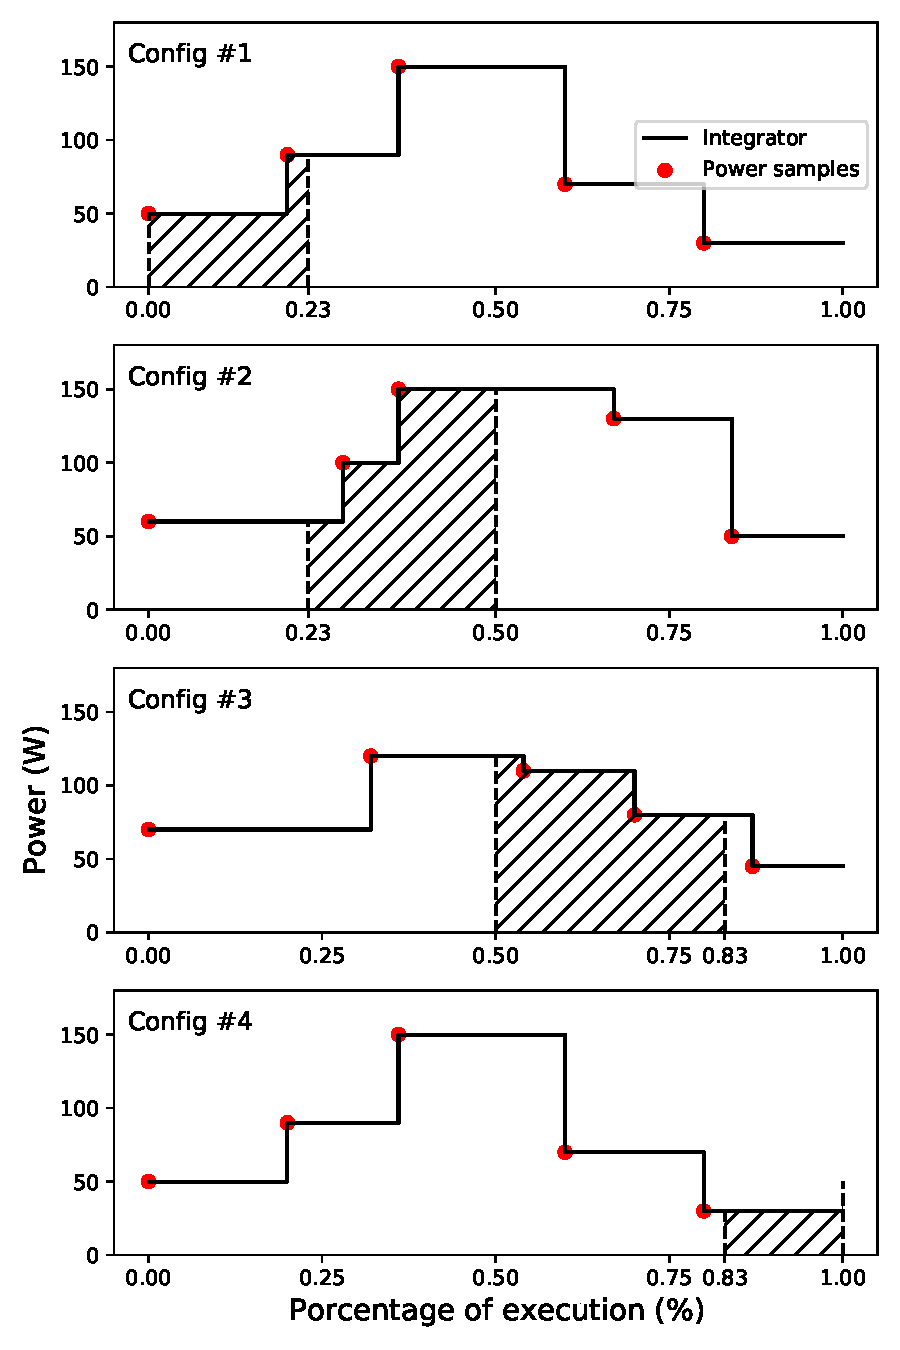
\includegraphics[width=\columnwidth]{phases/figures/integrator.pdf}
	\caption{Power vs percentage of execution for a given application in several configurations of power. The energy is represented by the hatched area.}
	\label{fig:zero_order}
\end{figure}

The pseudo-algorithm for the integrator is described below:

\begin{lstlisting}[language=c++]
	integrator(total_time, nsamples,
	times, powers
	begin_phase, end_phase)
	{
		energy = 0;
		ti = total_time * begin_phase; // initial time
		tf = total_time * end_phase; // final time
		
		idx_i = 0, idx_f = 0;
		
		// find the index of first sample in the range
		for (idx_i= 0; idx_i<nsamples; idx_i++)
		if (times[idx_i] >= ti)
		break;
		idx_i = (idx_i != 0) ? idx_i - 1 : 0;
		
		// find the index of last sample in the range
		for (idx_f= idx_i; i<nsamples; idx_f++)
		if (times[idx_f] >= tf)
		break;
		idx_f = (idx_f != 0) ? idx_f - 1 : 0;
		
		// in case there is only one sample
		if (idx_i == idx_f) 
		return (tf-ti)*powers[idx_i];
		
		// handle the edges
		energy=(times[idx_i+1]-ti)*powers[idx_i]
		energy+=(tf-times[idx_f])*powers[idx_f];
		
		// handle sample in between
		for (int i= idx_i+1; i<idx_f; i++)
		energy += (times[i+1]-times[i])*powers[i];
		
		return energy;
	}
\end{lstlisting}

To obtain an optimal energy configuration for a given phase division, we can run all possible configurations and select the one that leads to a minimal consumption, as shown in the pseudo-algorithm below:

\begin{lstlisting}
	phase_optimization(configs, phases)
	{
		total_en = 0;
		for (i = 0; i<phases.size(); i++)
		{
			min_en = -1;
			for (j = 0; j<configs.size(); j++)
			{
				en = estimate_energy_phase(
				configs[j].total_time, 
				configs[j].nsamples,
				configs[j].time_samples,
				configs[j].power_samples,
				phases[i], phases[i + 1]);
				if (min_en == -1 || en < min_en)
				{
					min_en = en;
					min_conf = configs[j];
				}
			}
			total_en += min_en;
		}
		return total_en;
	}
\end{lstlisting}

This method can now obtain an optimal energy configuration for a given phase. The next step is to find the best phase, division.

\section{Results} \label{sec:results}

Now that we can evaluate phase divisions, we need to answer two questions, what is the best number of phases, and what is the best division within this number?

For that, we used the algorithm described previously in \cref{sec:heuristic} as the objective of a minimization problem where we want to find the vector of phases that minimizes the total energy. Moreover, by using a genetic algorithm, we can accelerate the process by controlling mutation and initial population generation since we already know some information about our problem.

For instance, we decide to start studying phases in the range of 3 to 100 divisions. We used a GA with a population of $10^3$ individuals. We kept the best 10\% individuals on each generation while having a 10\% of mutation rate, running for 300 generations. The reproduction function for the GA combines half-phases of one individual with another, and the mutation will randomly change a division.

We use the applications described in \cref{subsec:casestudyapplication}, to compute the optimal phase selection. The \cref{fig:relative_energy} shows the relative energy consumption compared to an optimized single phase.

\begin{figure}[H]
	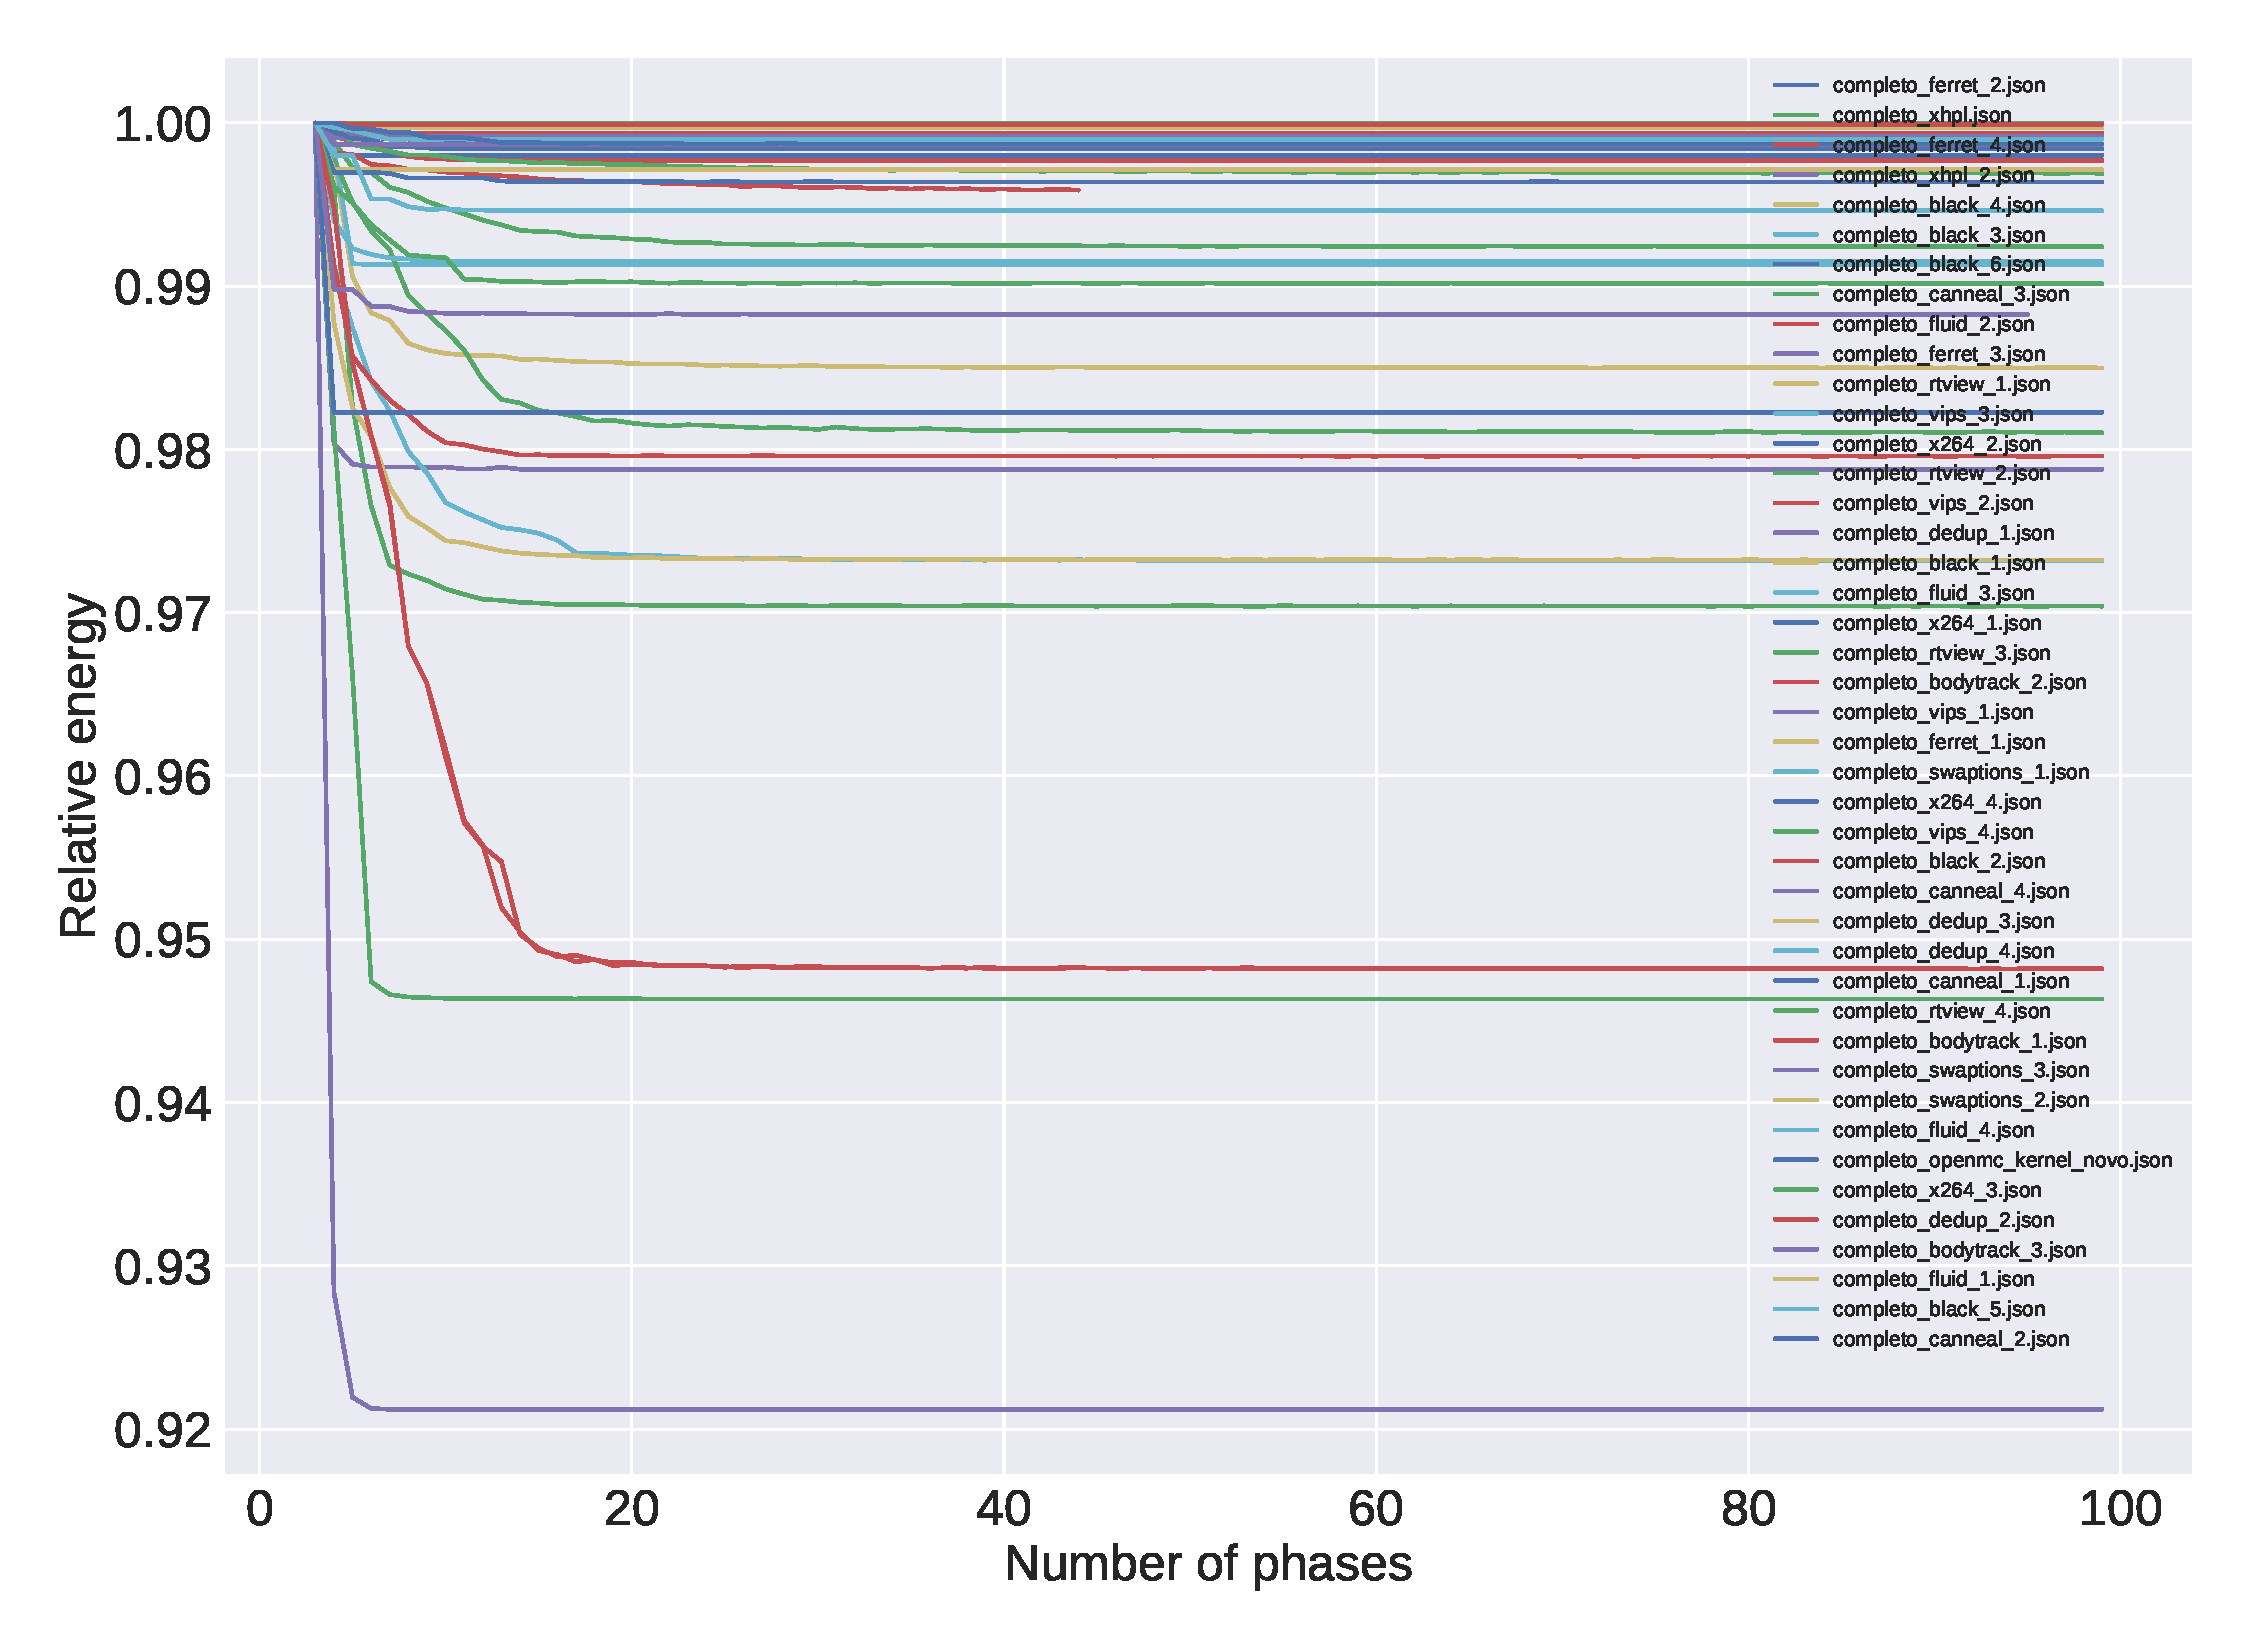
\includegraphics[width=\columnwidth]{fingerprint/figures/energy_per_phase.pdf}
	\caption{Relative energy vs number of phases using applications from PARSEC 3.0, HPC, and Openmc benchmarks with different inputs. Energy compared to the single-phase optimal configuration.}
	\label{fig:relative_energy}
\end{figure}

This evaluation shows very interesting results, as shown in \cref{fig:relative_energy}. An ideal single-phase configuration provides the highest energy consumption for all cases. Furthermore, dividing the application into more than 35 phases is not necessary. On average, power consumption stopped after 35 phases.

% \begin{figure}[H]
% 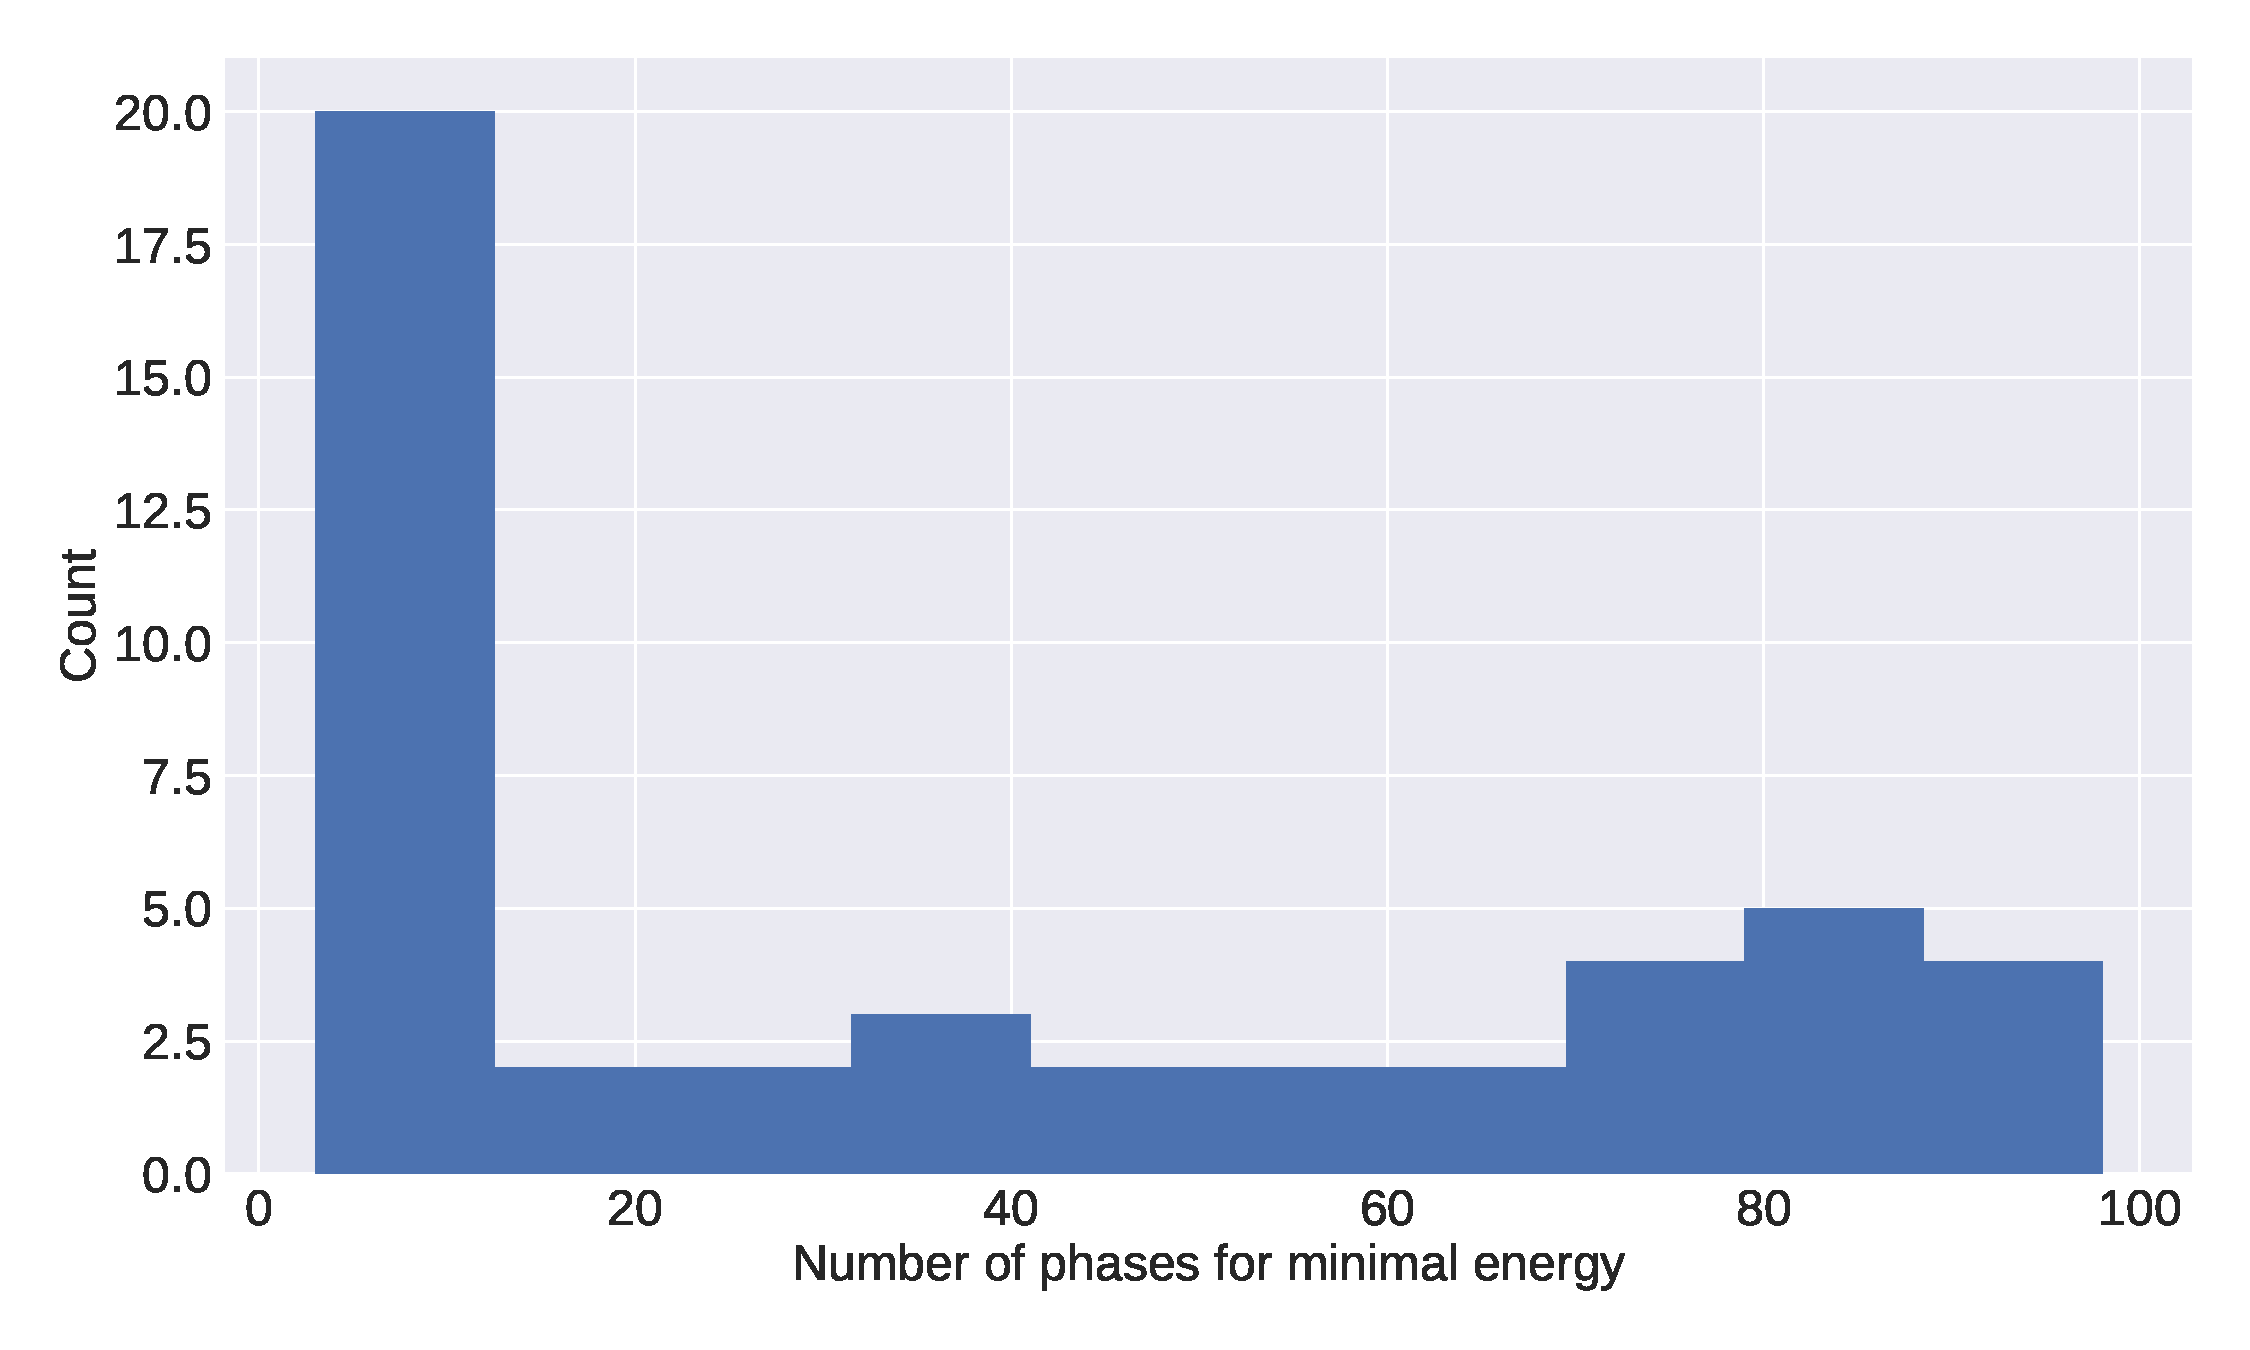
\includegraphics[width=\columnwidth]{figures/min_phases_distribution.pdf}
%     \caption{Histogram of minimal number of phases to optimal energy}
%     \label{fig:hist_optimal_phase}
% \end{figure}

The results meet our expectation that the optimum of n-divisions phases will always be better than or equal to n-1 divisions. This becomes clearer when we look at the number of cores, and frequency curve \cref{fig:freq_control} and \cref{fig:cores_control}, since starting from a certain number of divisions does not change the control signals since dividing an ideal phase into two would result in two phases with the same control signals. Therefore, the energy will remain the same, and there is no reason to increase the number of phases beyond that.

\begin{figure}[h]
	\centering
	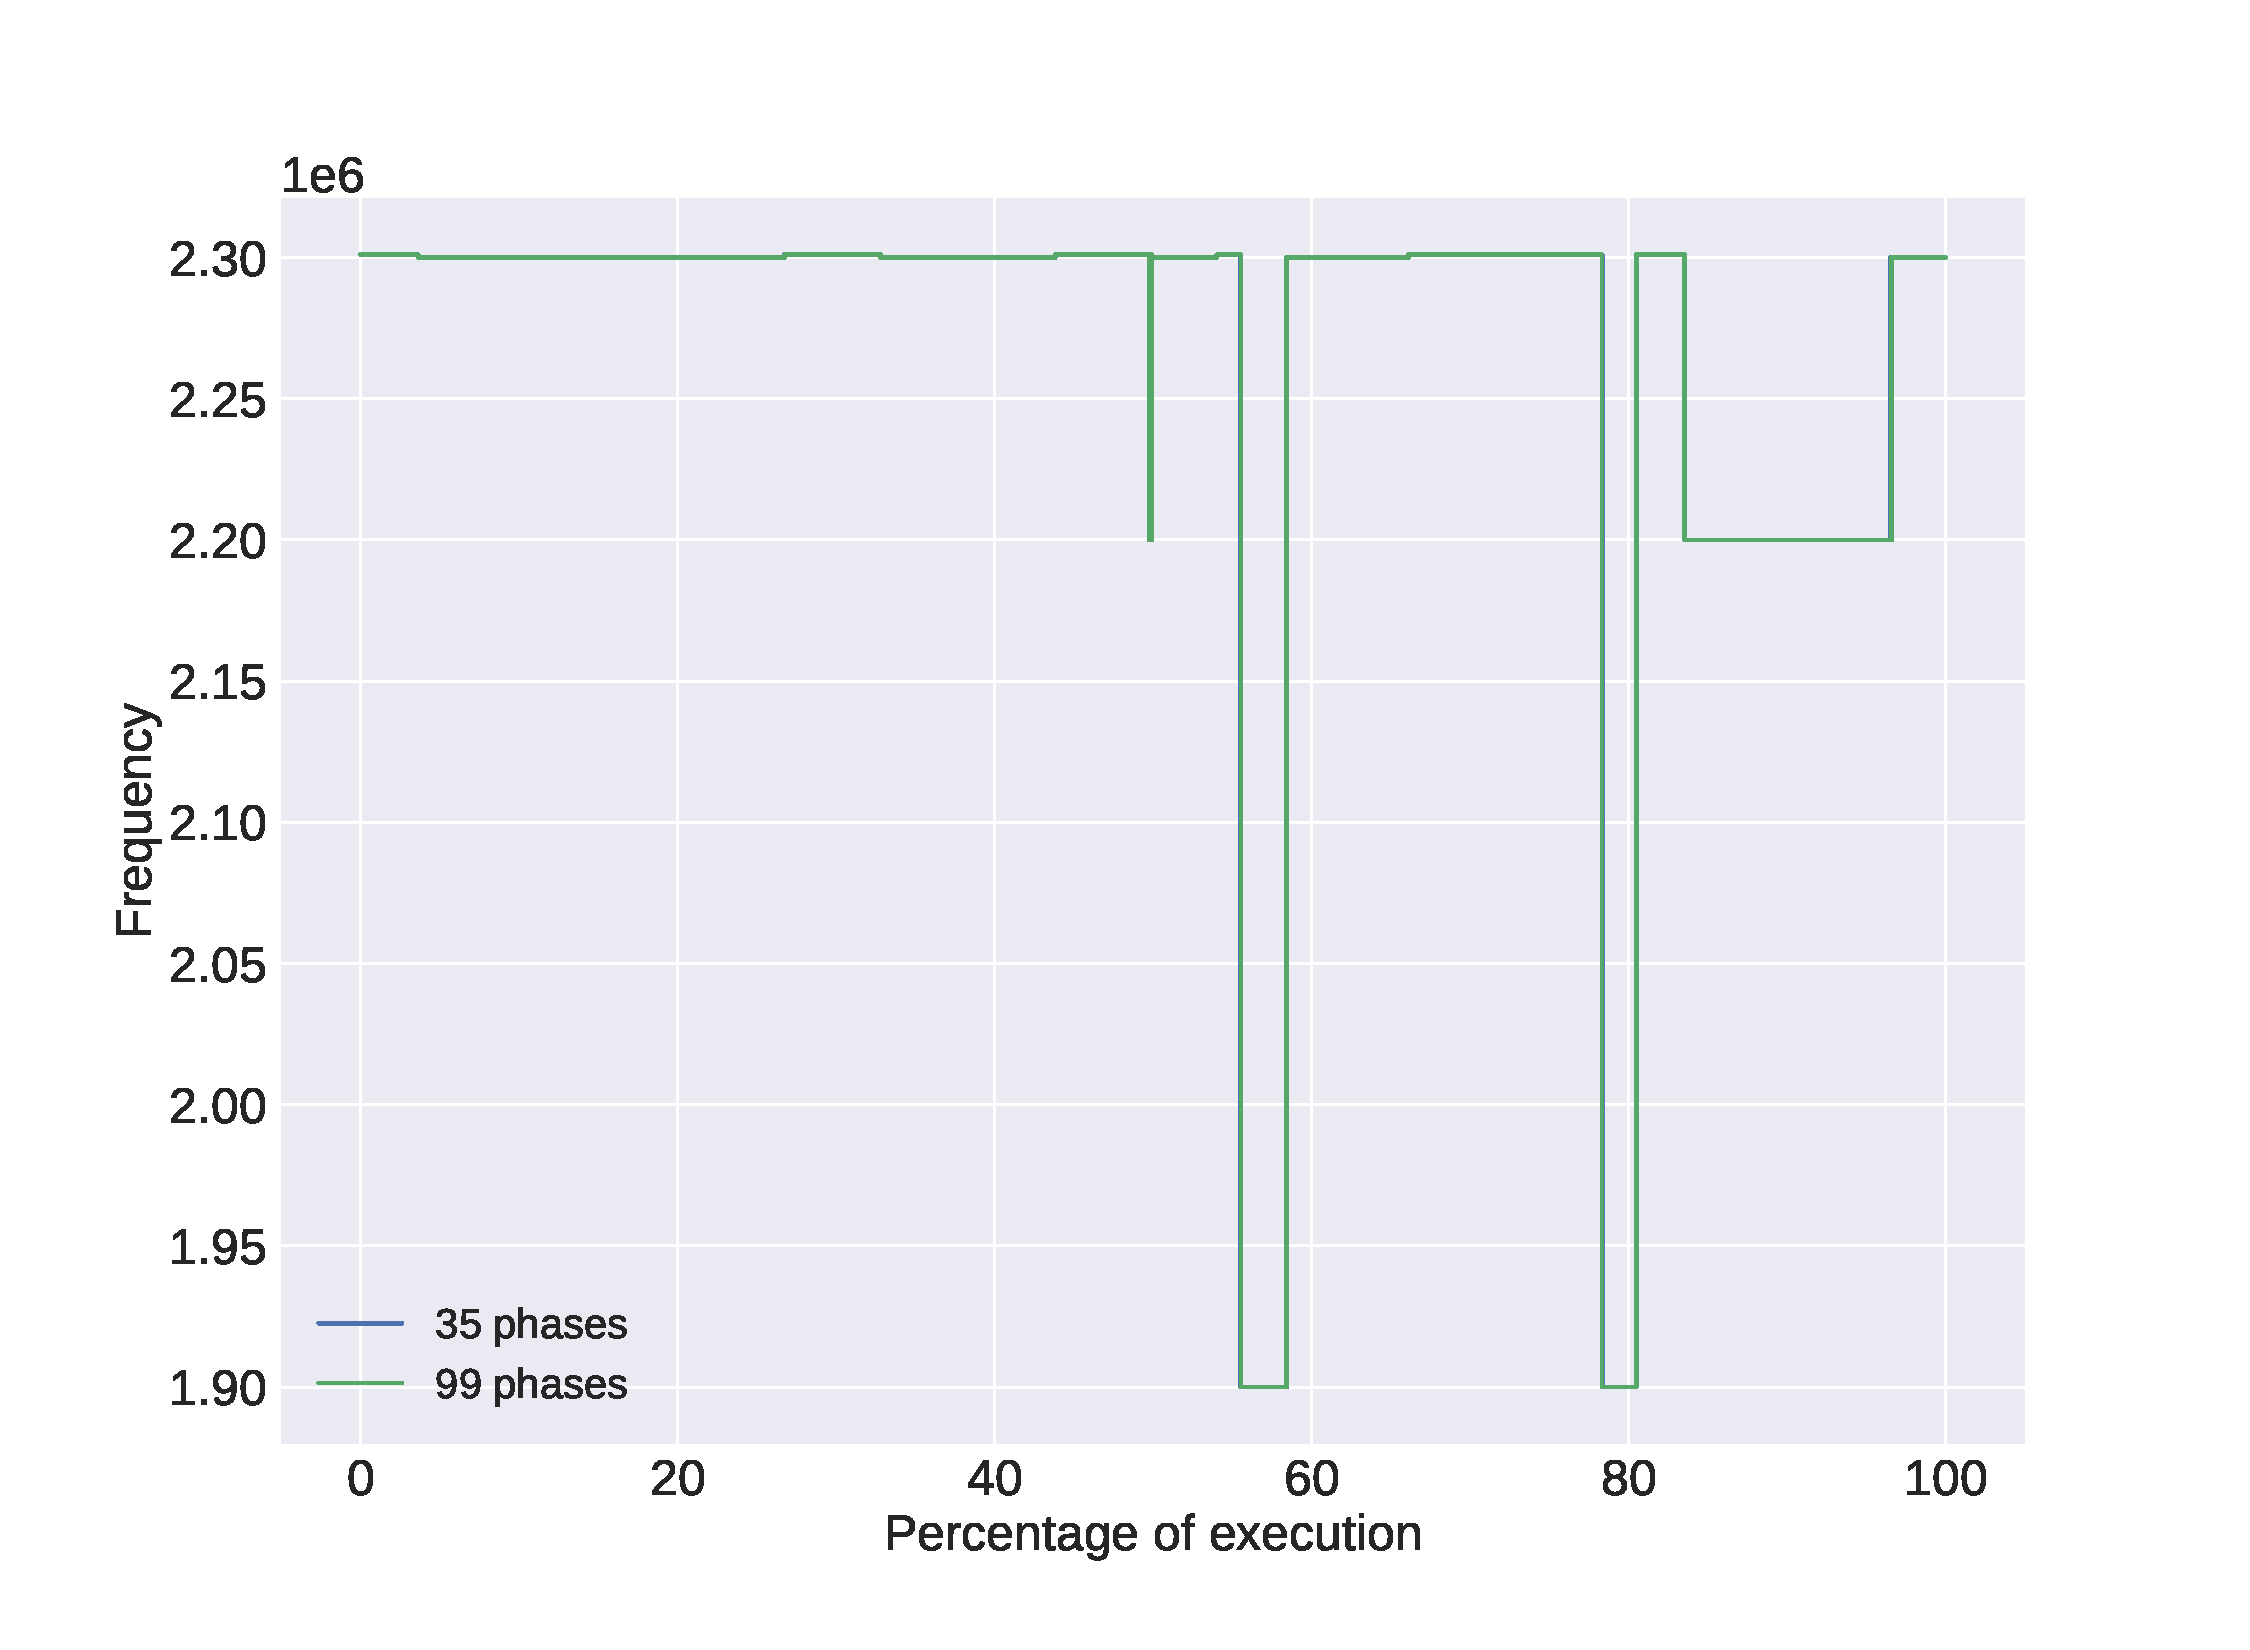
\includegraphics[width=\columnwidth]{phases/figures/signals/completo_bodytrack_1_freq_signals_cmp.pdf}
	\caption{Frequency signal vs percentage of execution for the Bodytrack application, comparing the difference of 35 and 99 phases.}
\end{figure}%

\begin{figure}[h]
	\centering
	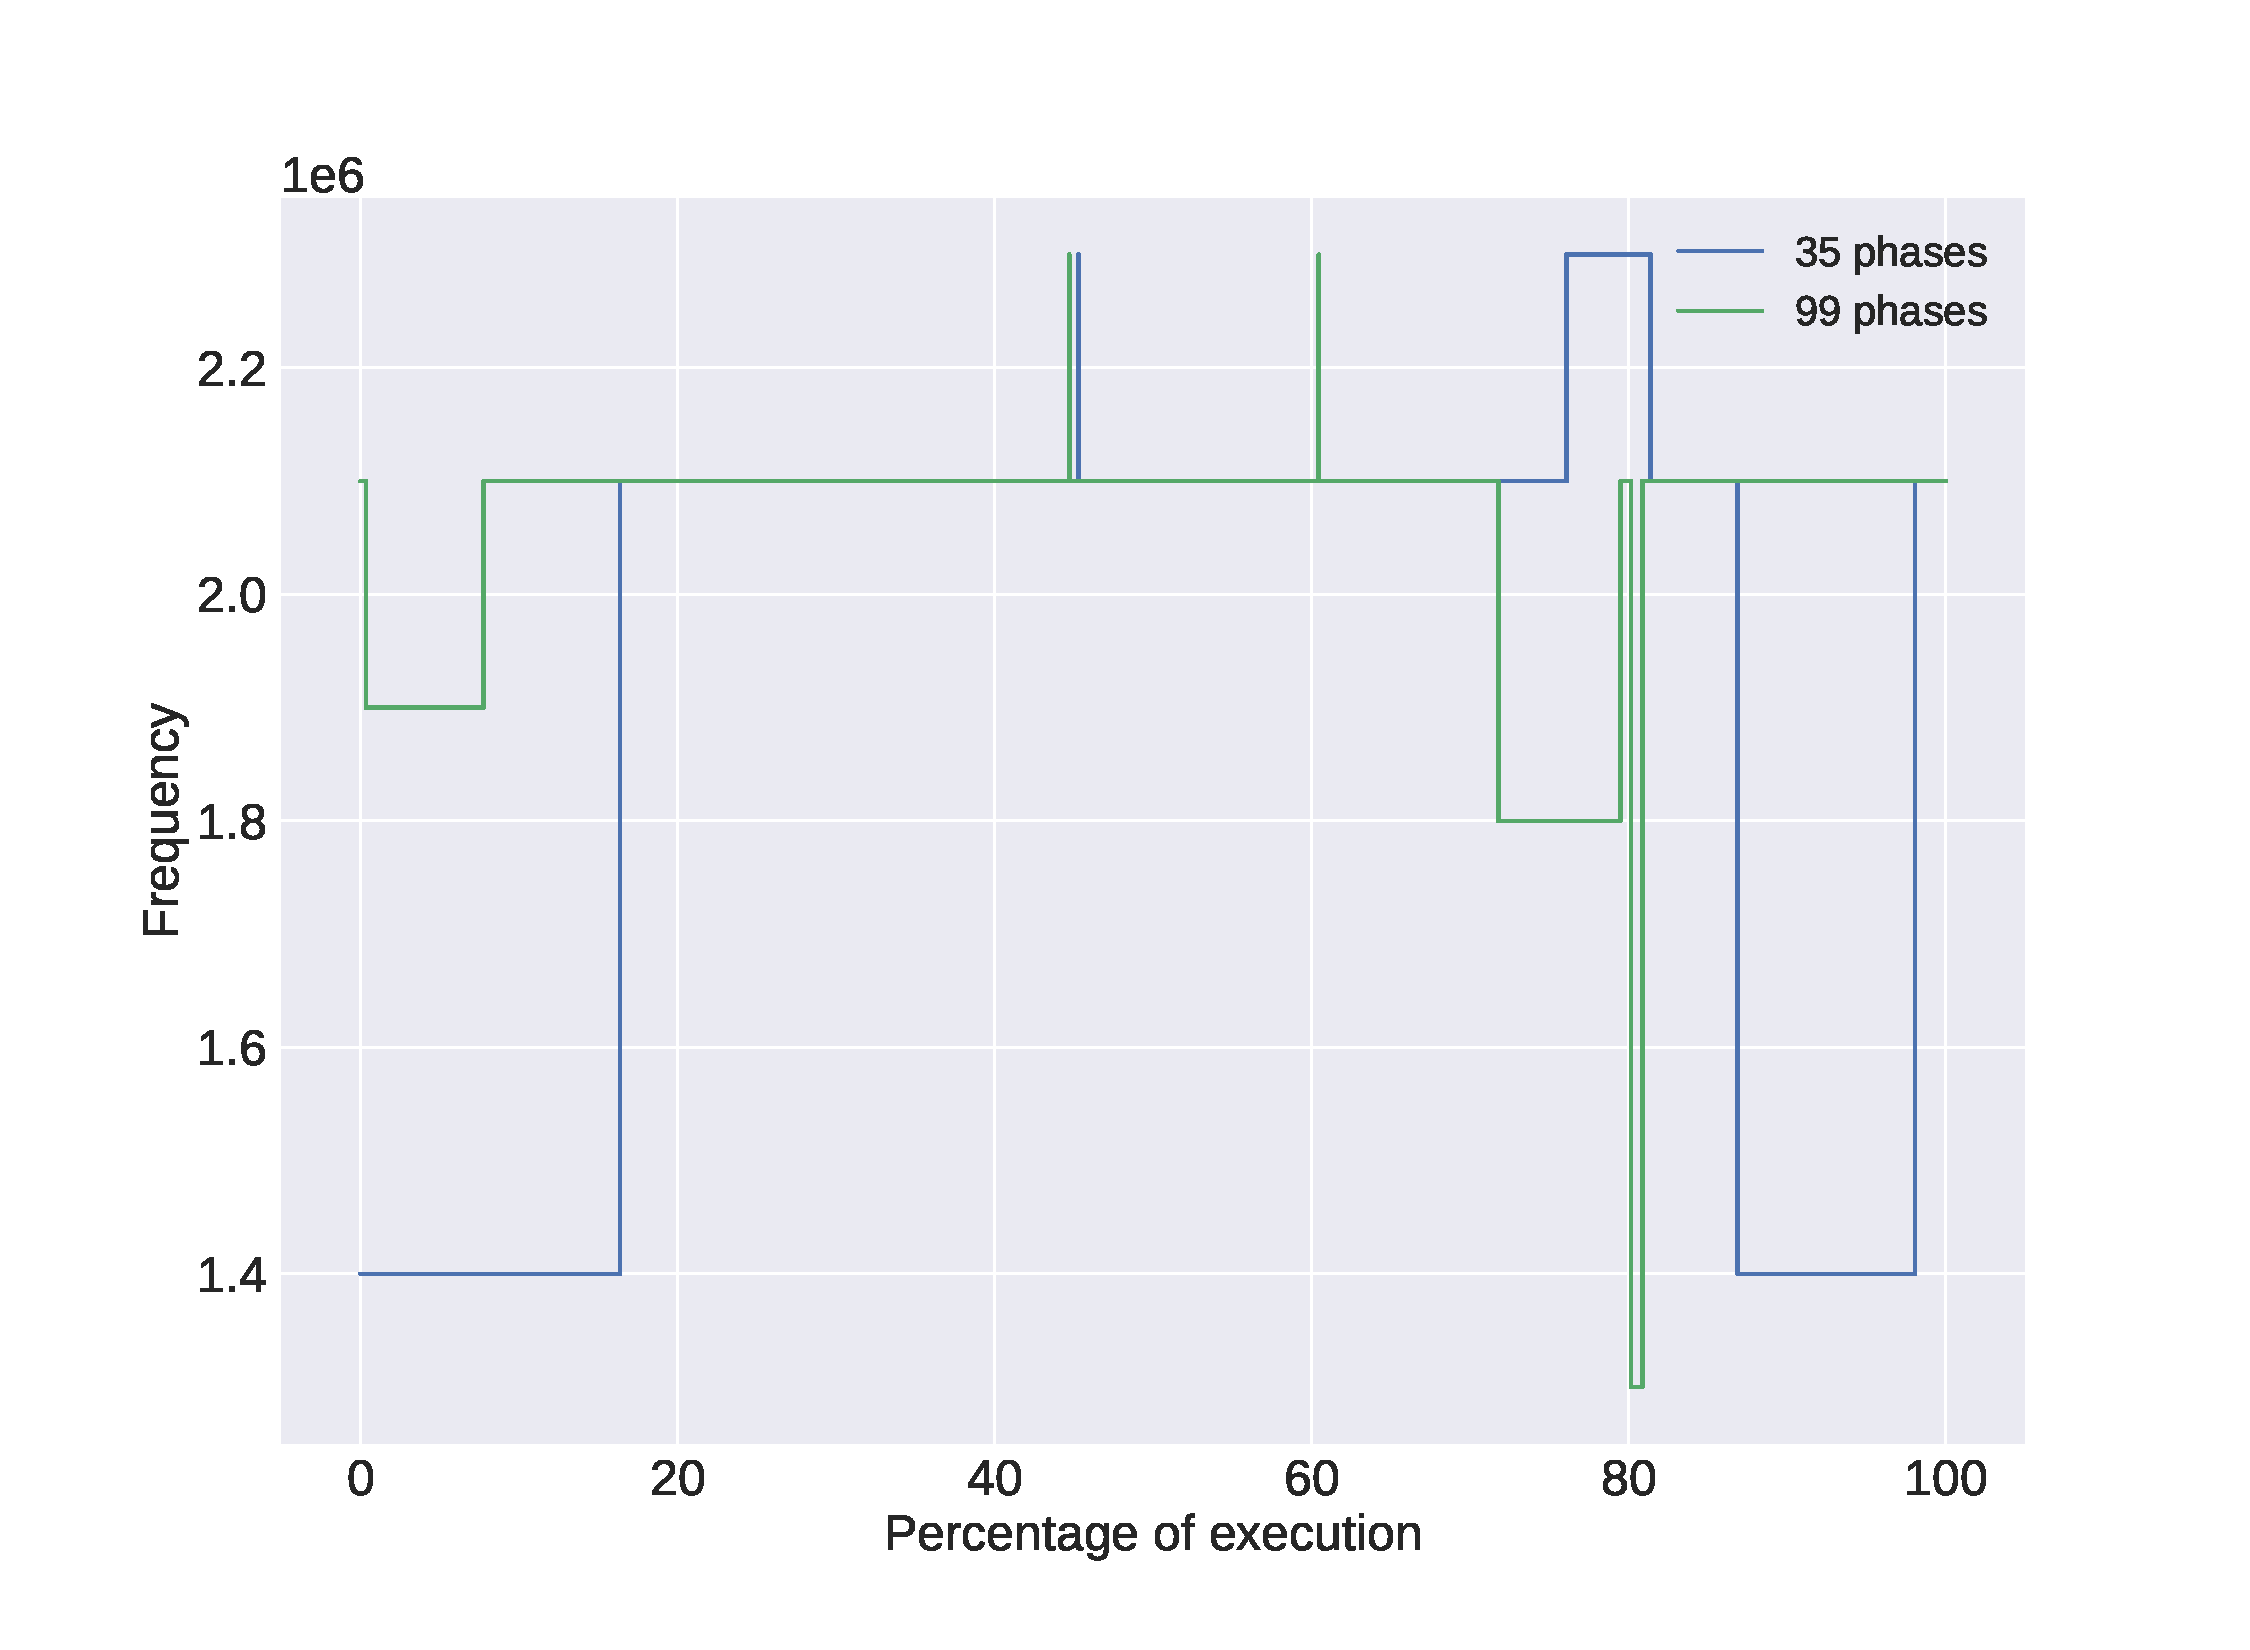
\includegraphics[width=\columnwidth]{phases/figures/signals/completo_freq_freq_signals_cmp.pdf}
	\caption{Frequency signal vs percentage of execution for the Freqmine application, comparing the difference of 35 and 99 phases.}
\end{figure}%

\begin{figure}[h]
	\centering
	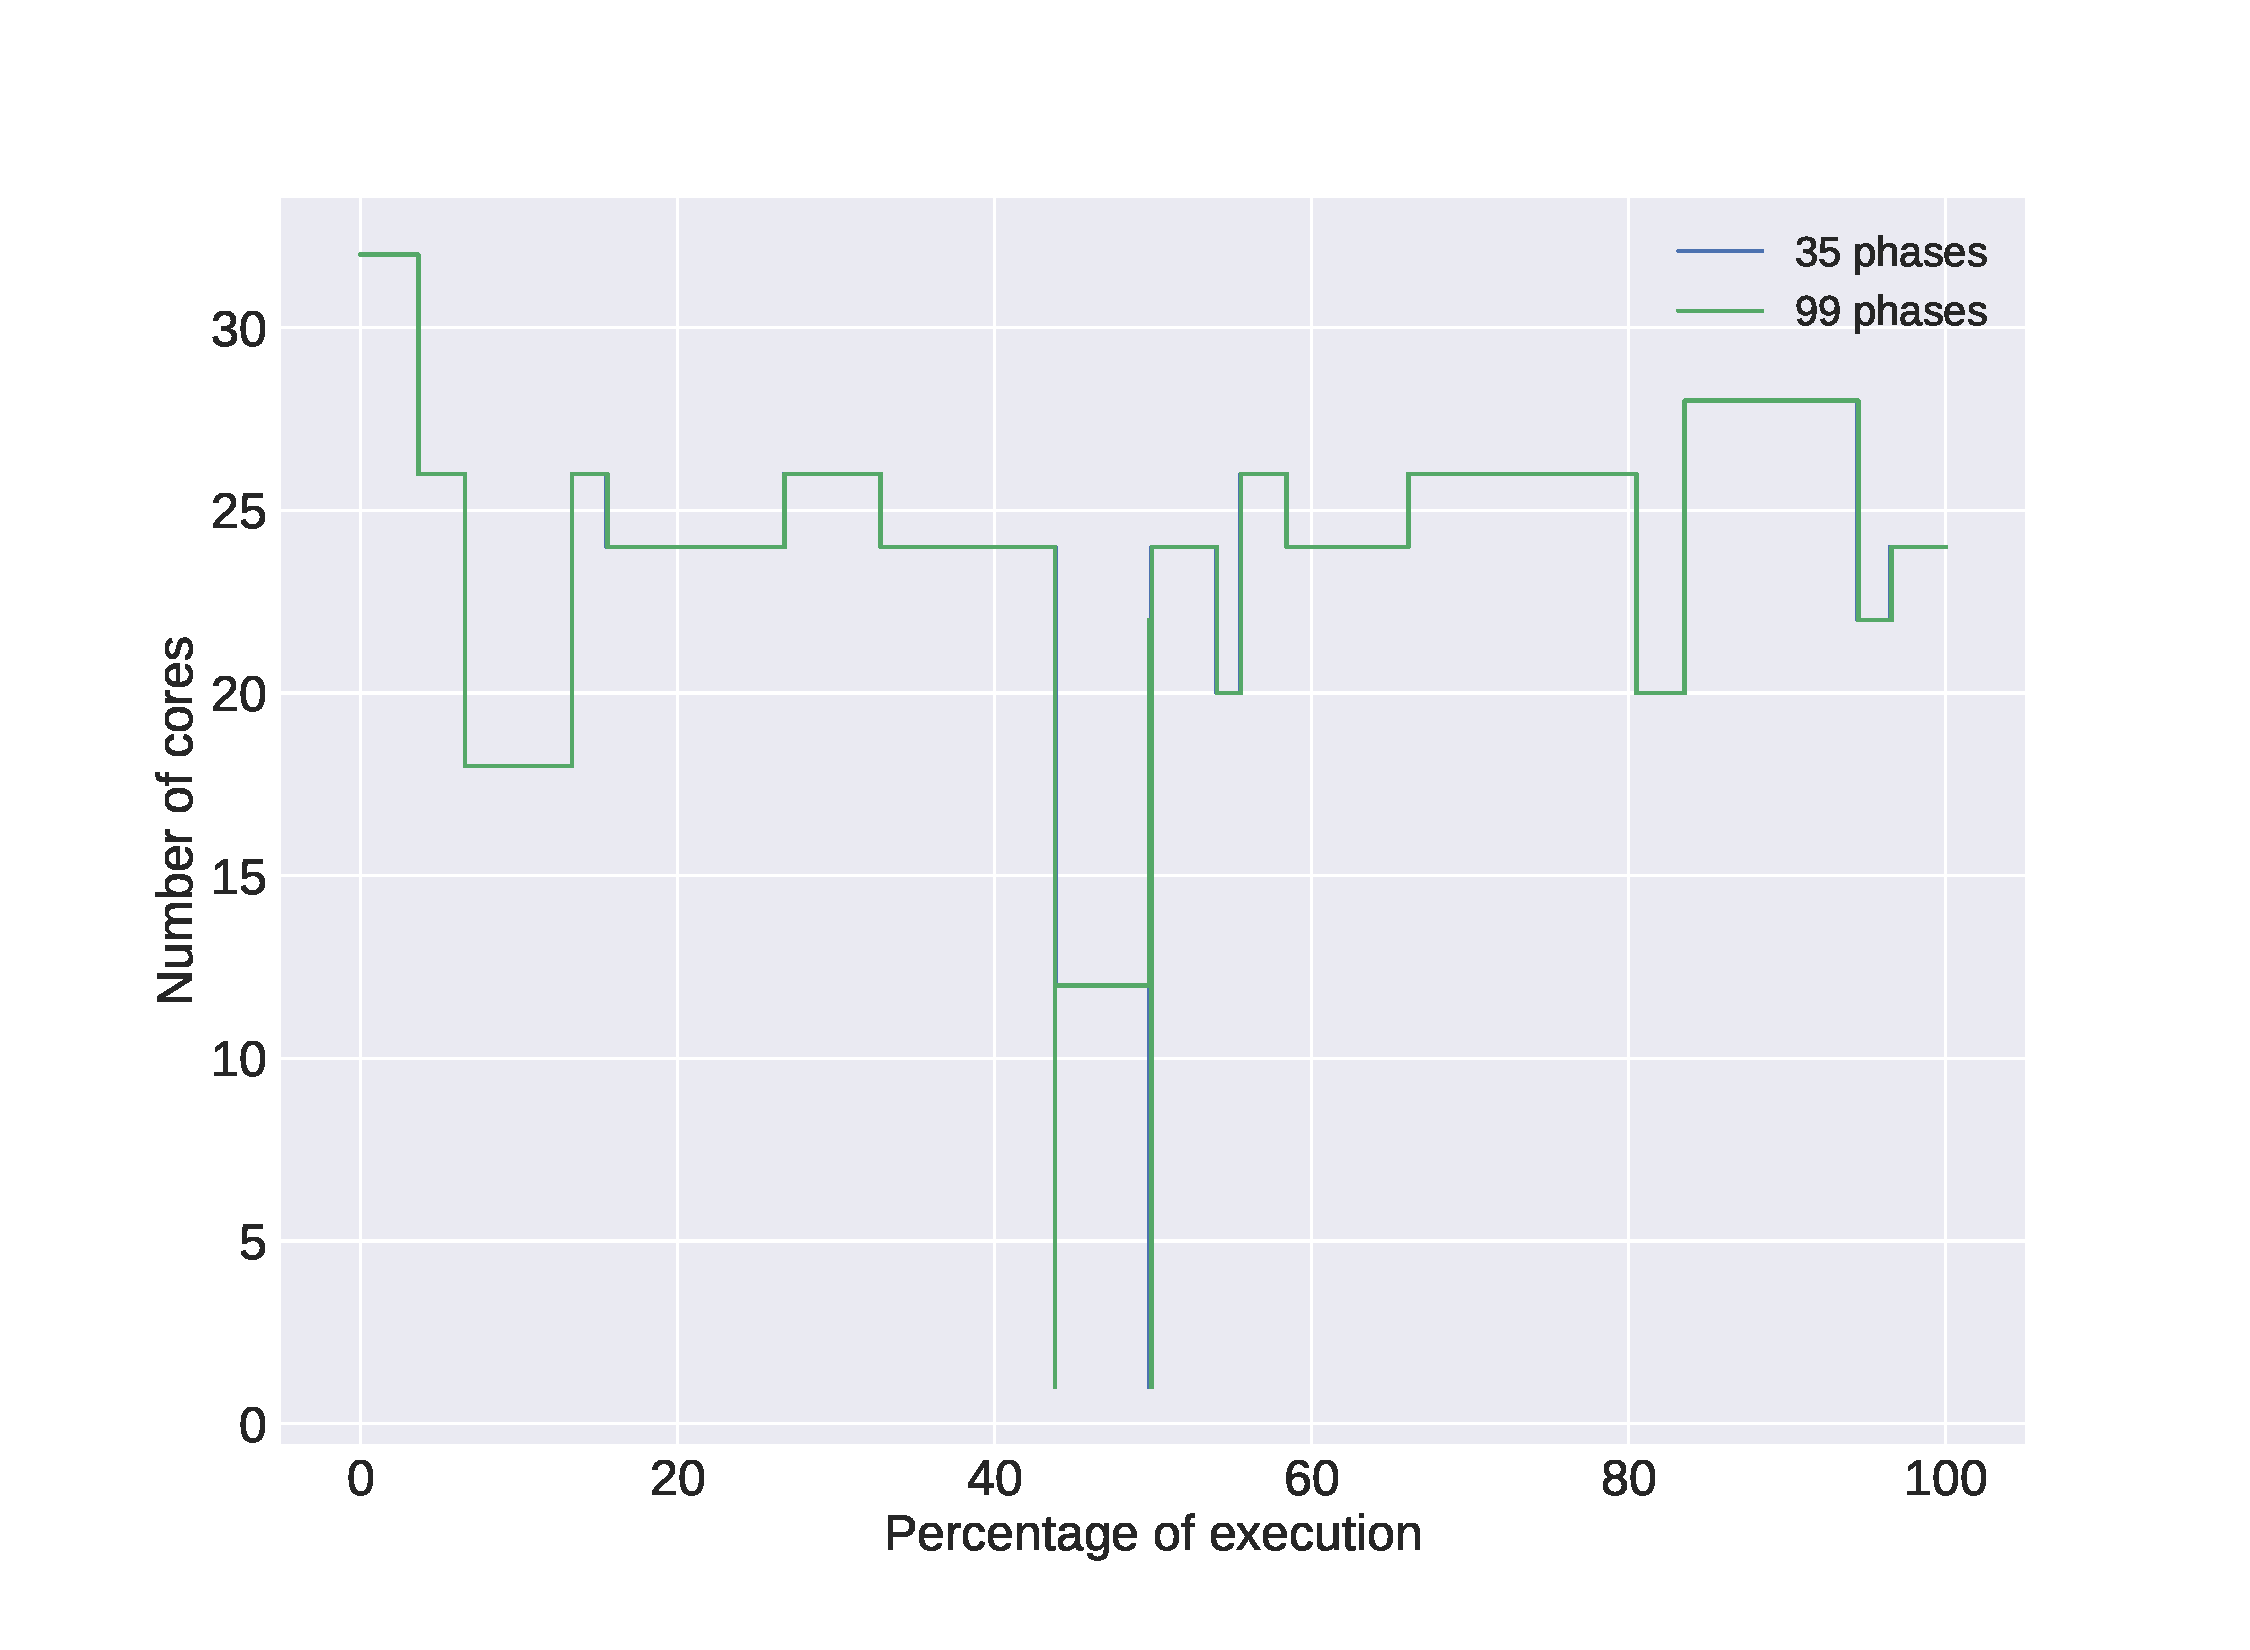
\includegraphics[width=\columnwidth]{phases/figures/signals/completo_bodytrack_1_cores_signals_cmp.pdf}
	\caption{Cores signal vs percentage of execution for the Bodytrack application, comparing the difference of 35 and 99 phases.}
\end{figure}%
\begin{figure}[h]
	\centering
	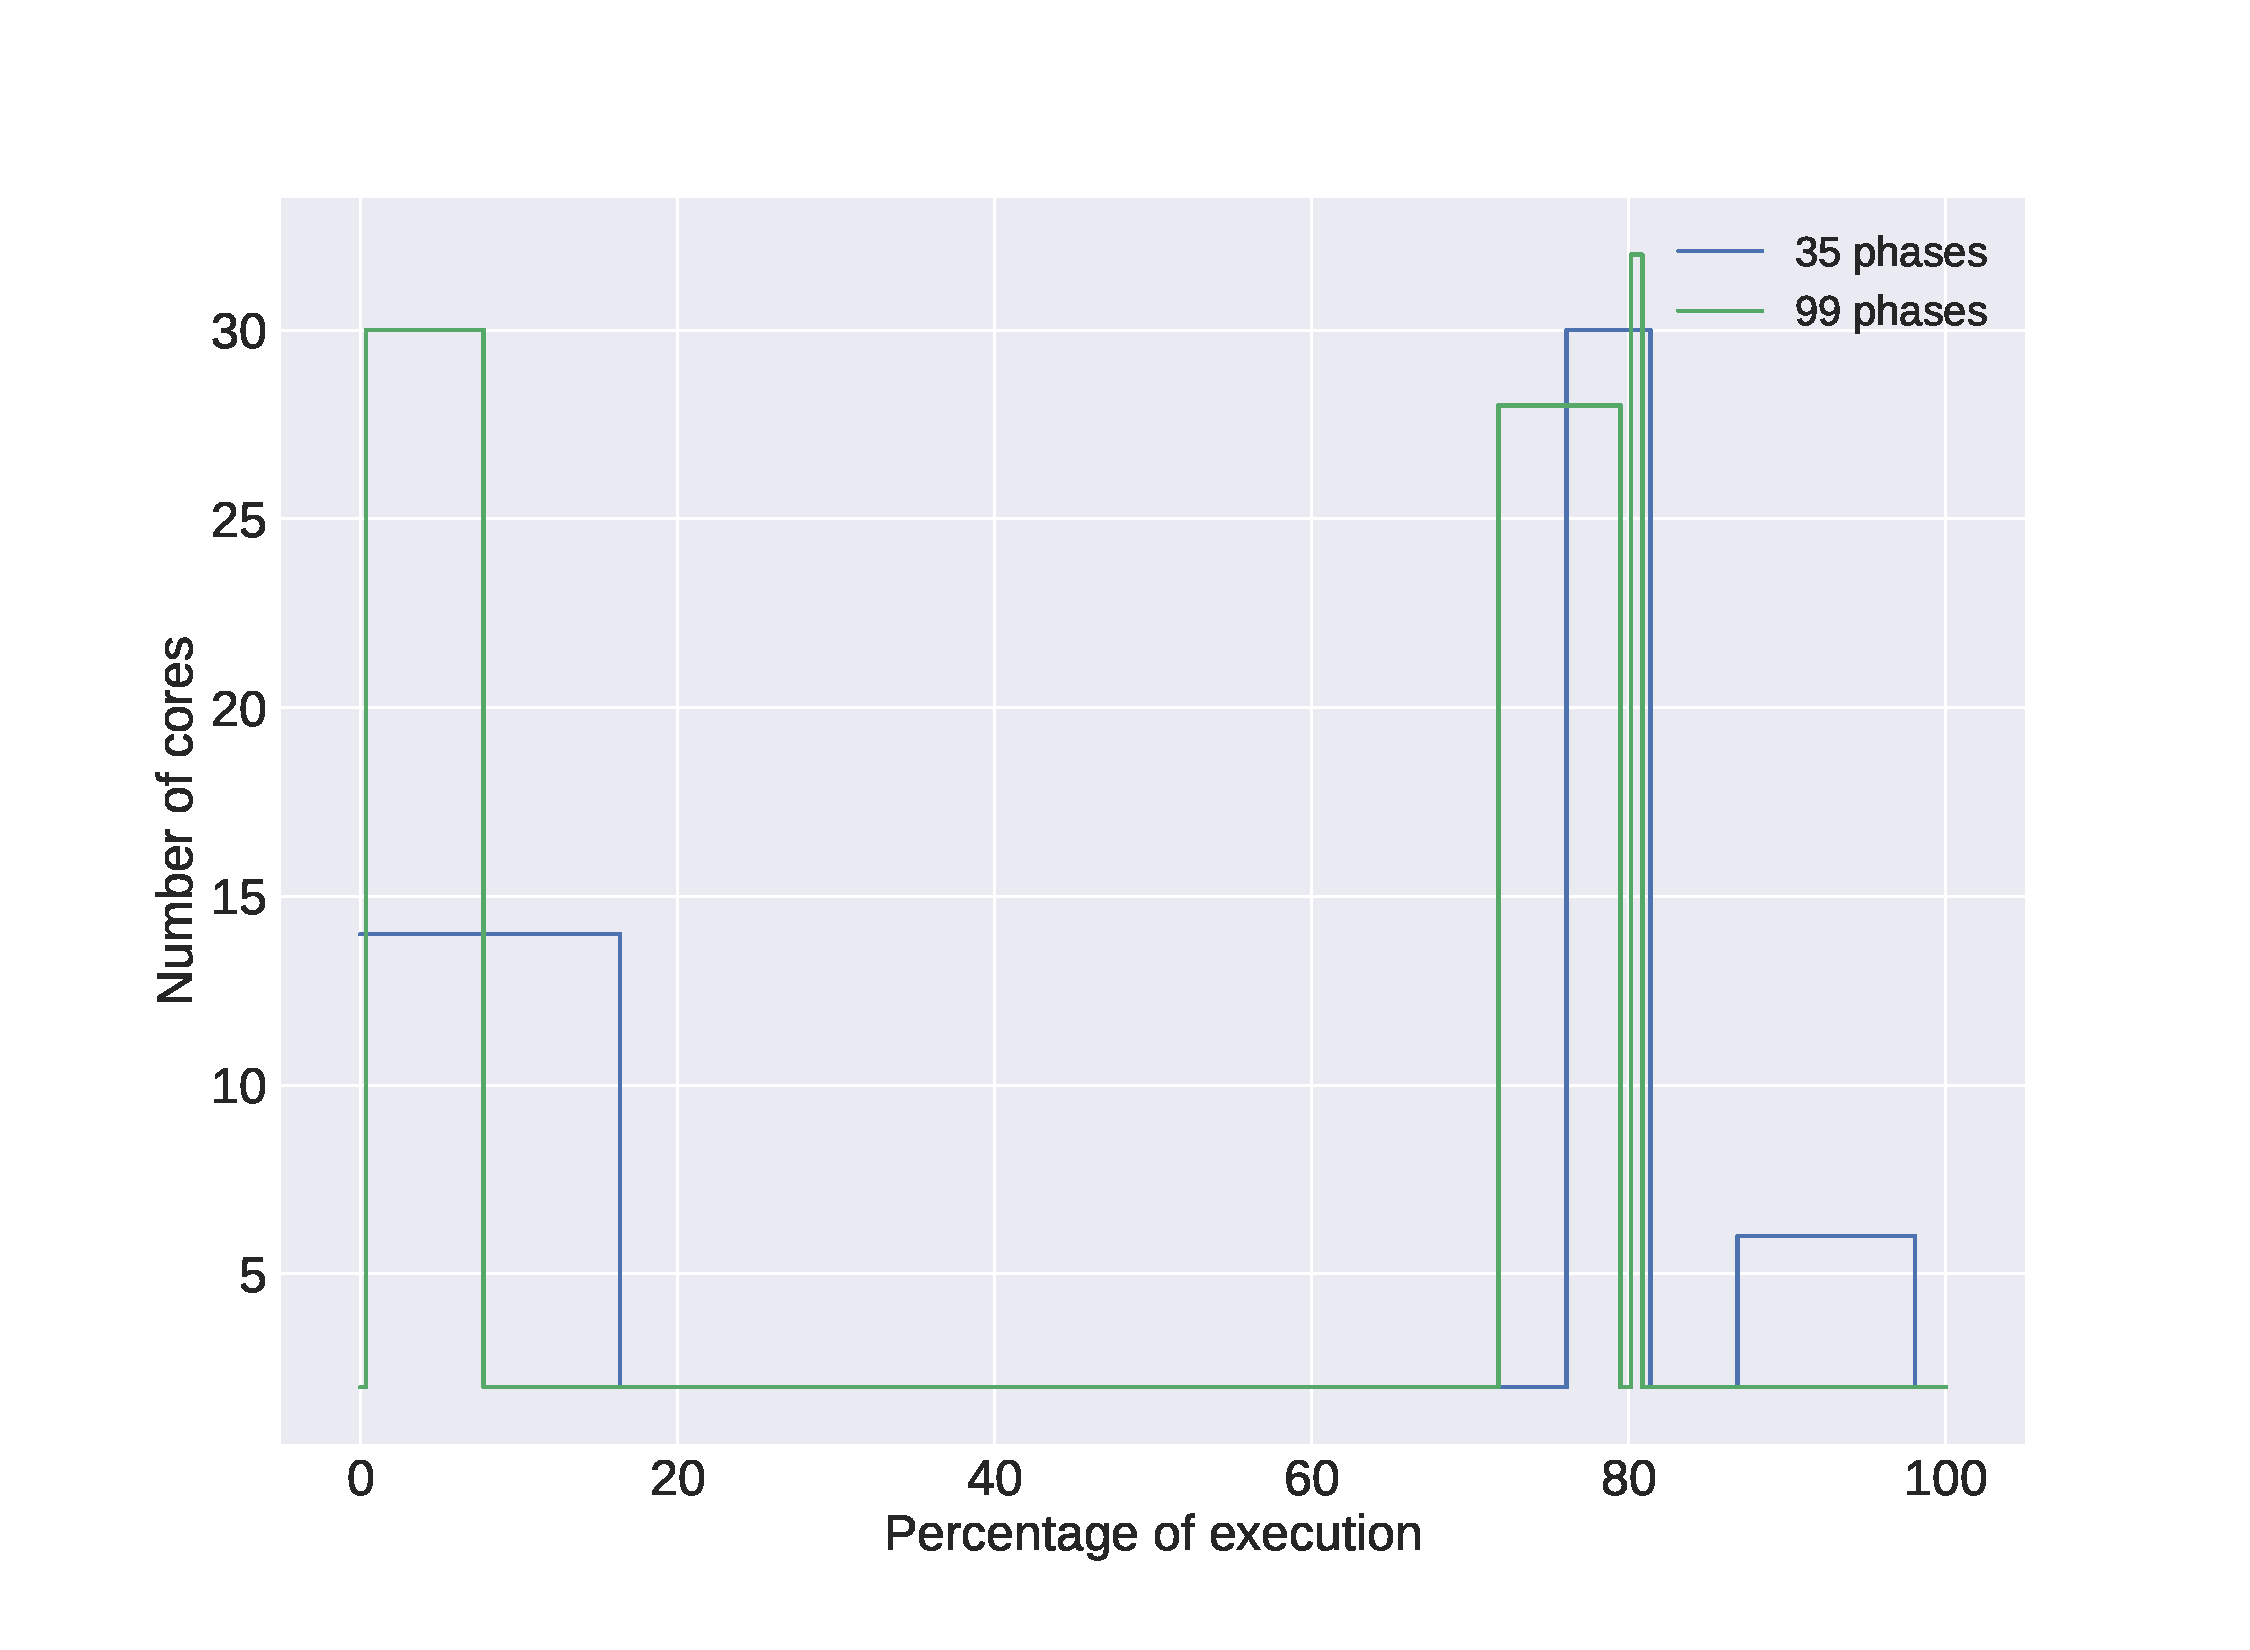
\includegraphics[width=\columnwidth]{phases/figures/signals/completo_freq_cores_signals_cmp.pdf}
	\caption{Cores signal vs percentage of execution for the Freqmine application, comparing the difference of 35 and 99 phases.}
\end{figure}%

When we compare this method with the default DVFS algorithm in Linux, we observer an average saving of 38\% as shown in \cref{fig:cmp_ondemand} the relative energy per application.

\begin{figure}[H]
	\centering
	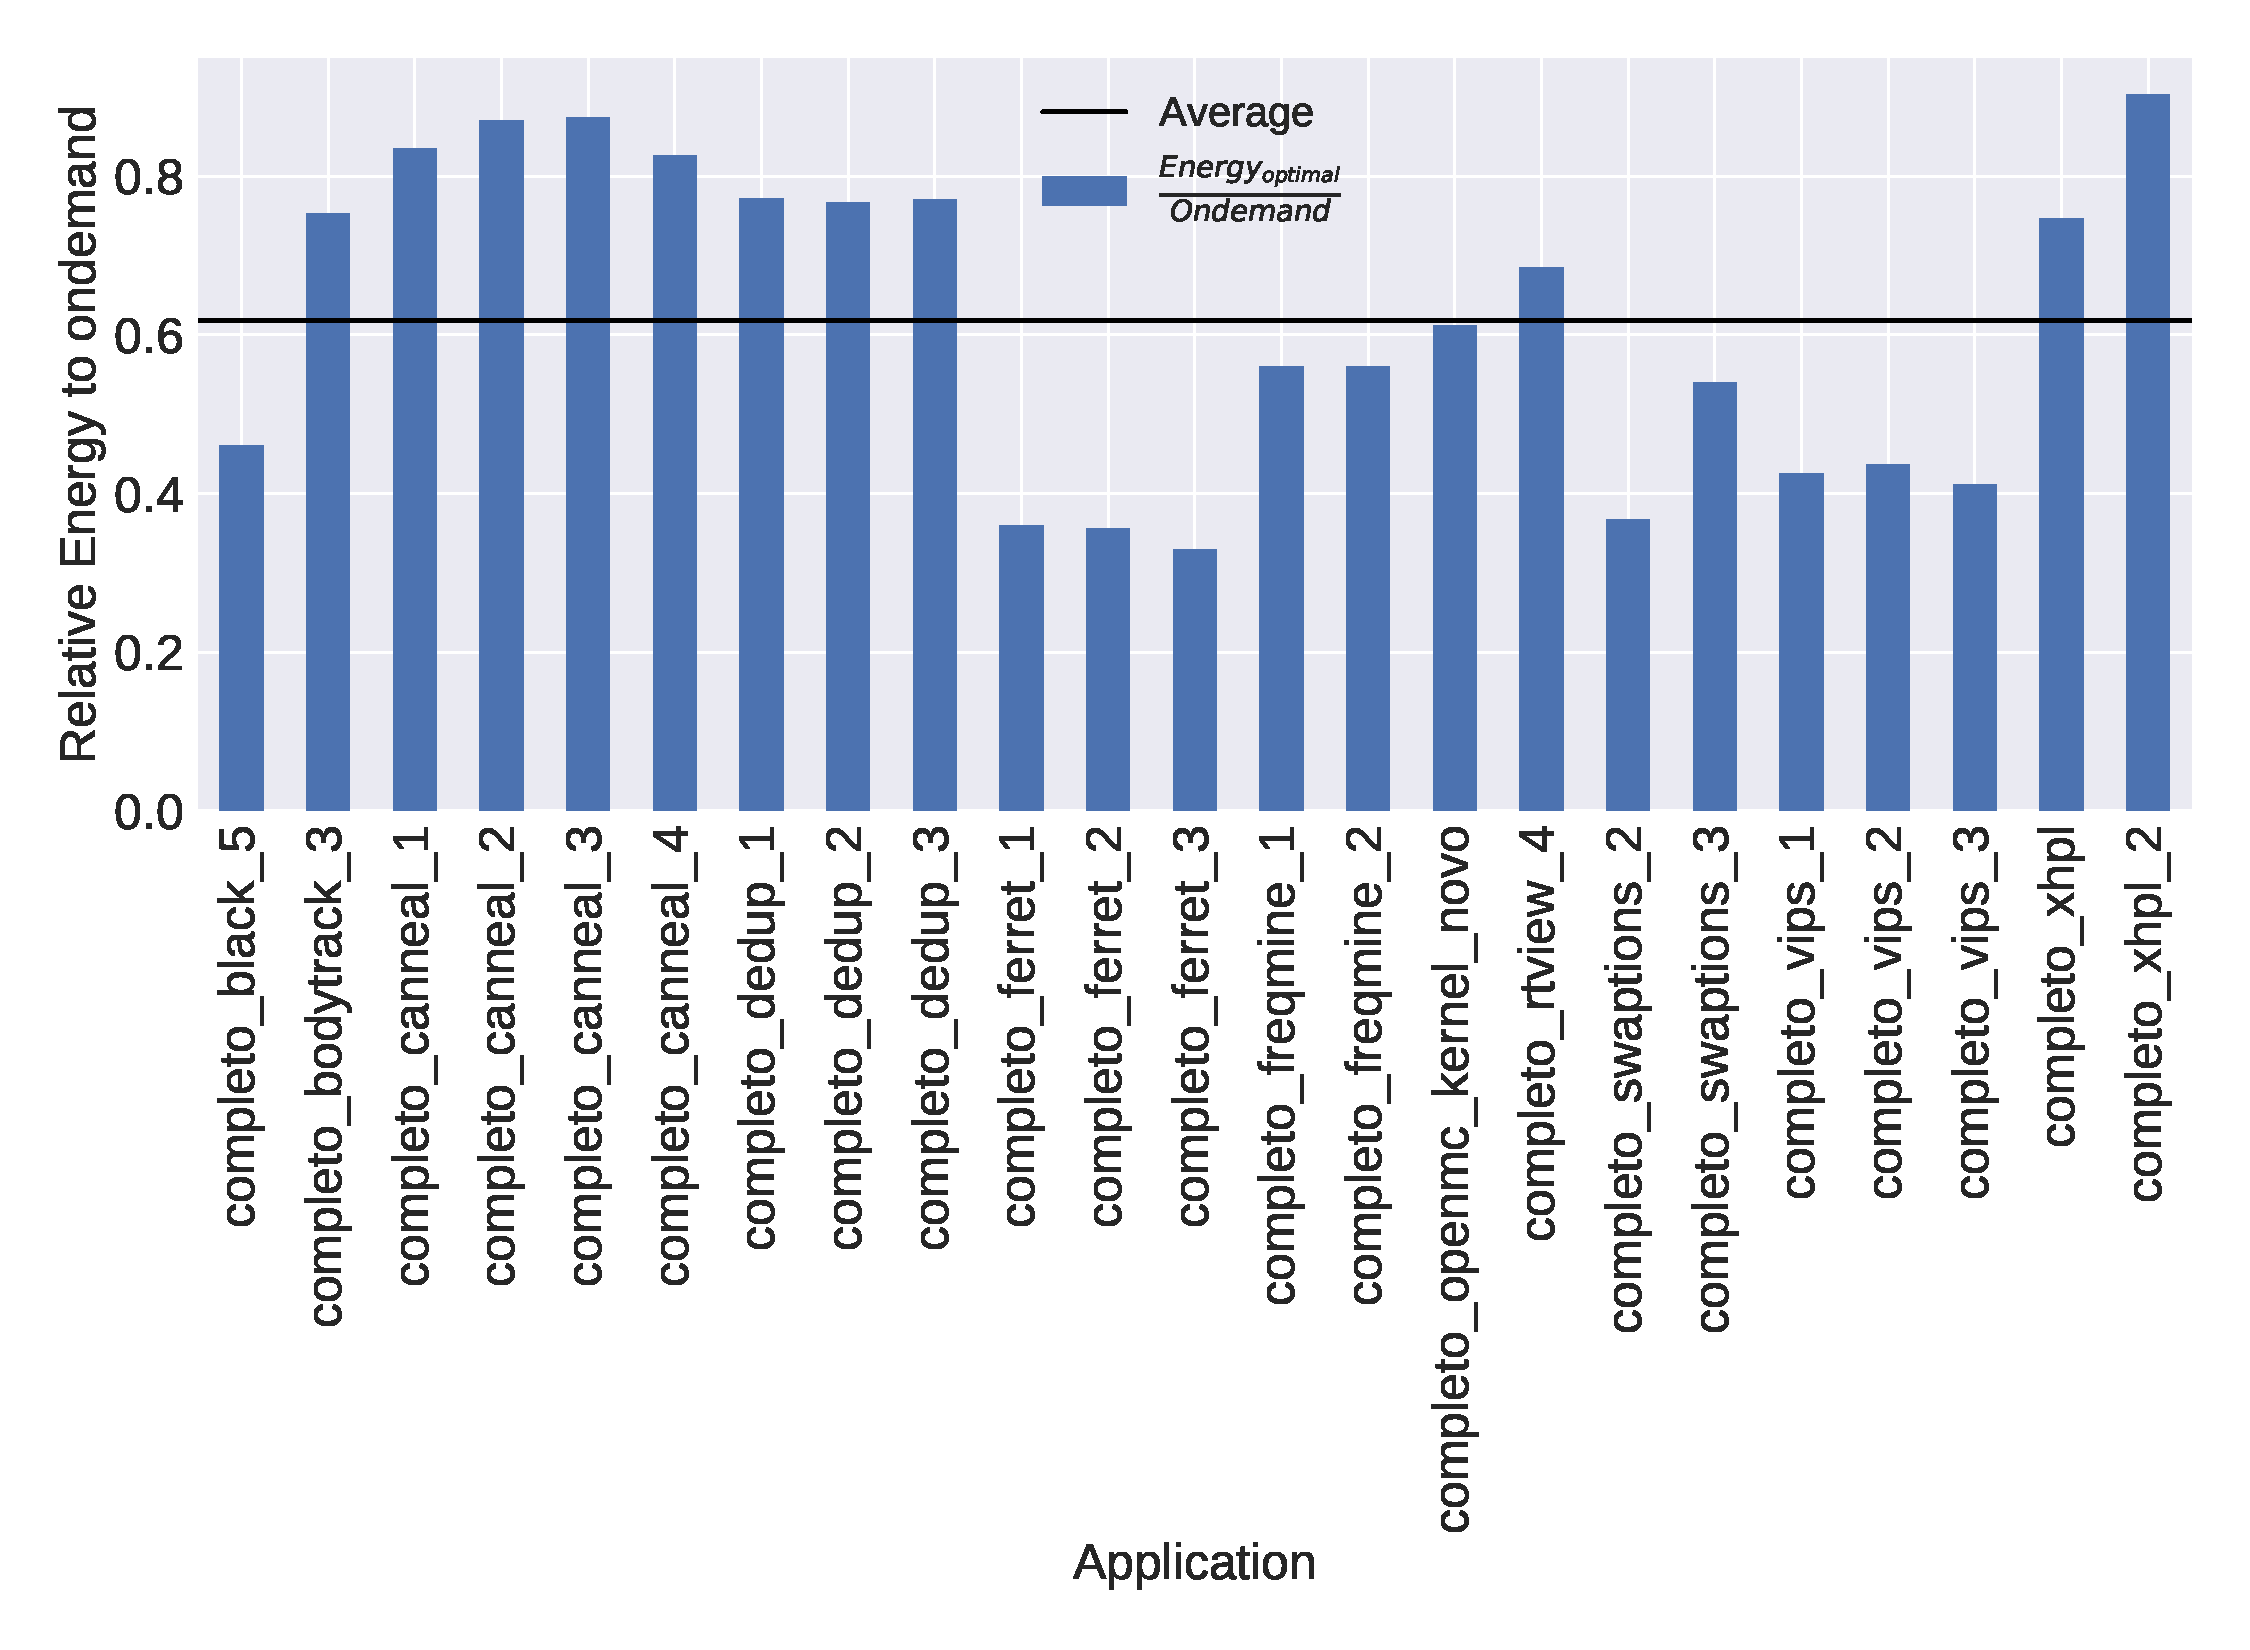
\includegraphics[width=\columnwidth]{phases/figures/comparison_ondemand.pdf}
	\caption{Relative energy comparison, optimal phase division energy compared to governor Ondemand on Linux.}
	\label{fig:cmp_ondemand}
\end{figure}

To illustrate the phases division, the \cref{fig:phase_division_cmap_35} and \cref{fig:phase_division_cmap_35} shows a heatmap with the divisions by application and the percentage of total energy spent in that phase. There we can see a pattern of 3 phases which for these applications are generally setup phase where it loads data from the disk, a computation phase where the data is processed, and a finalization phase where data is written back to the disk or displayed to the user.

\begin{figure}[H]
	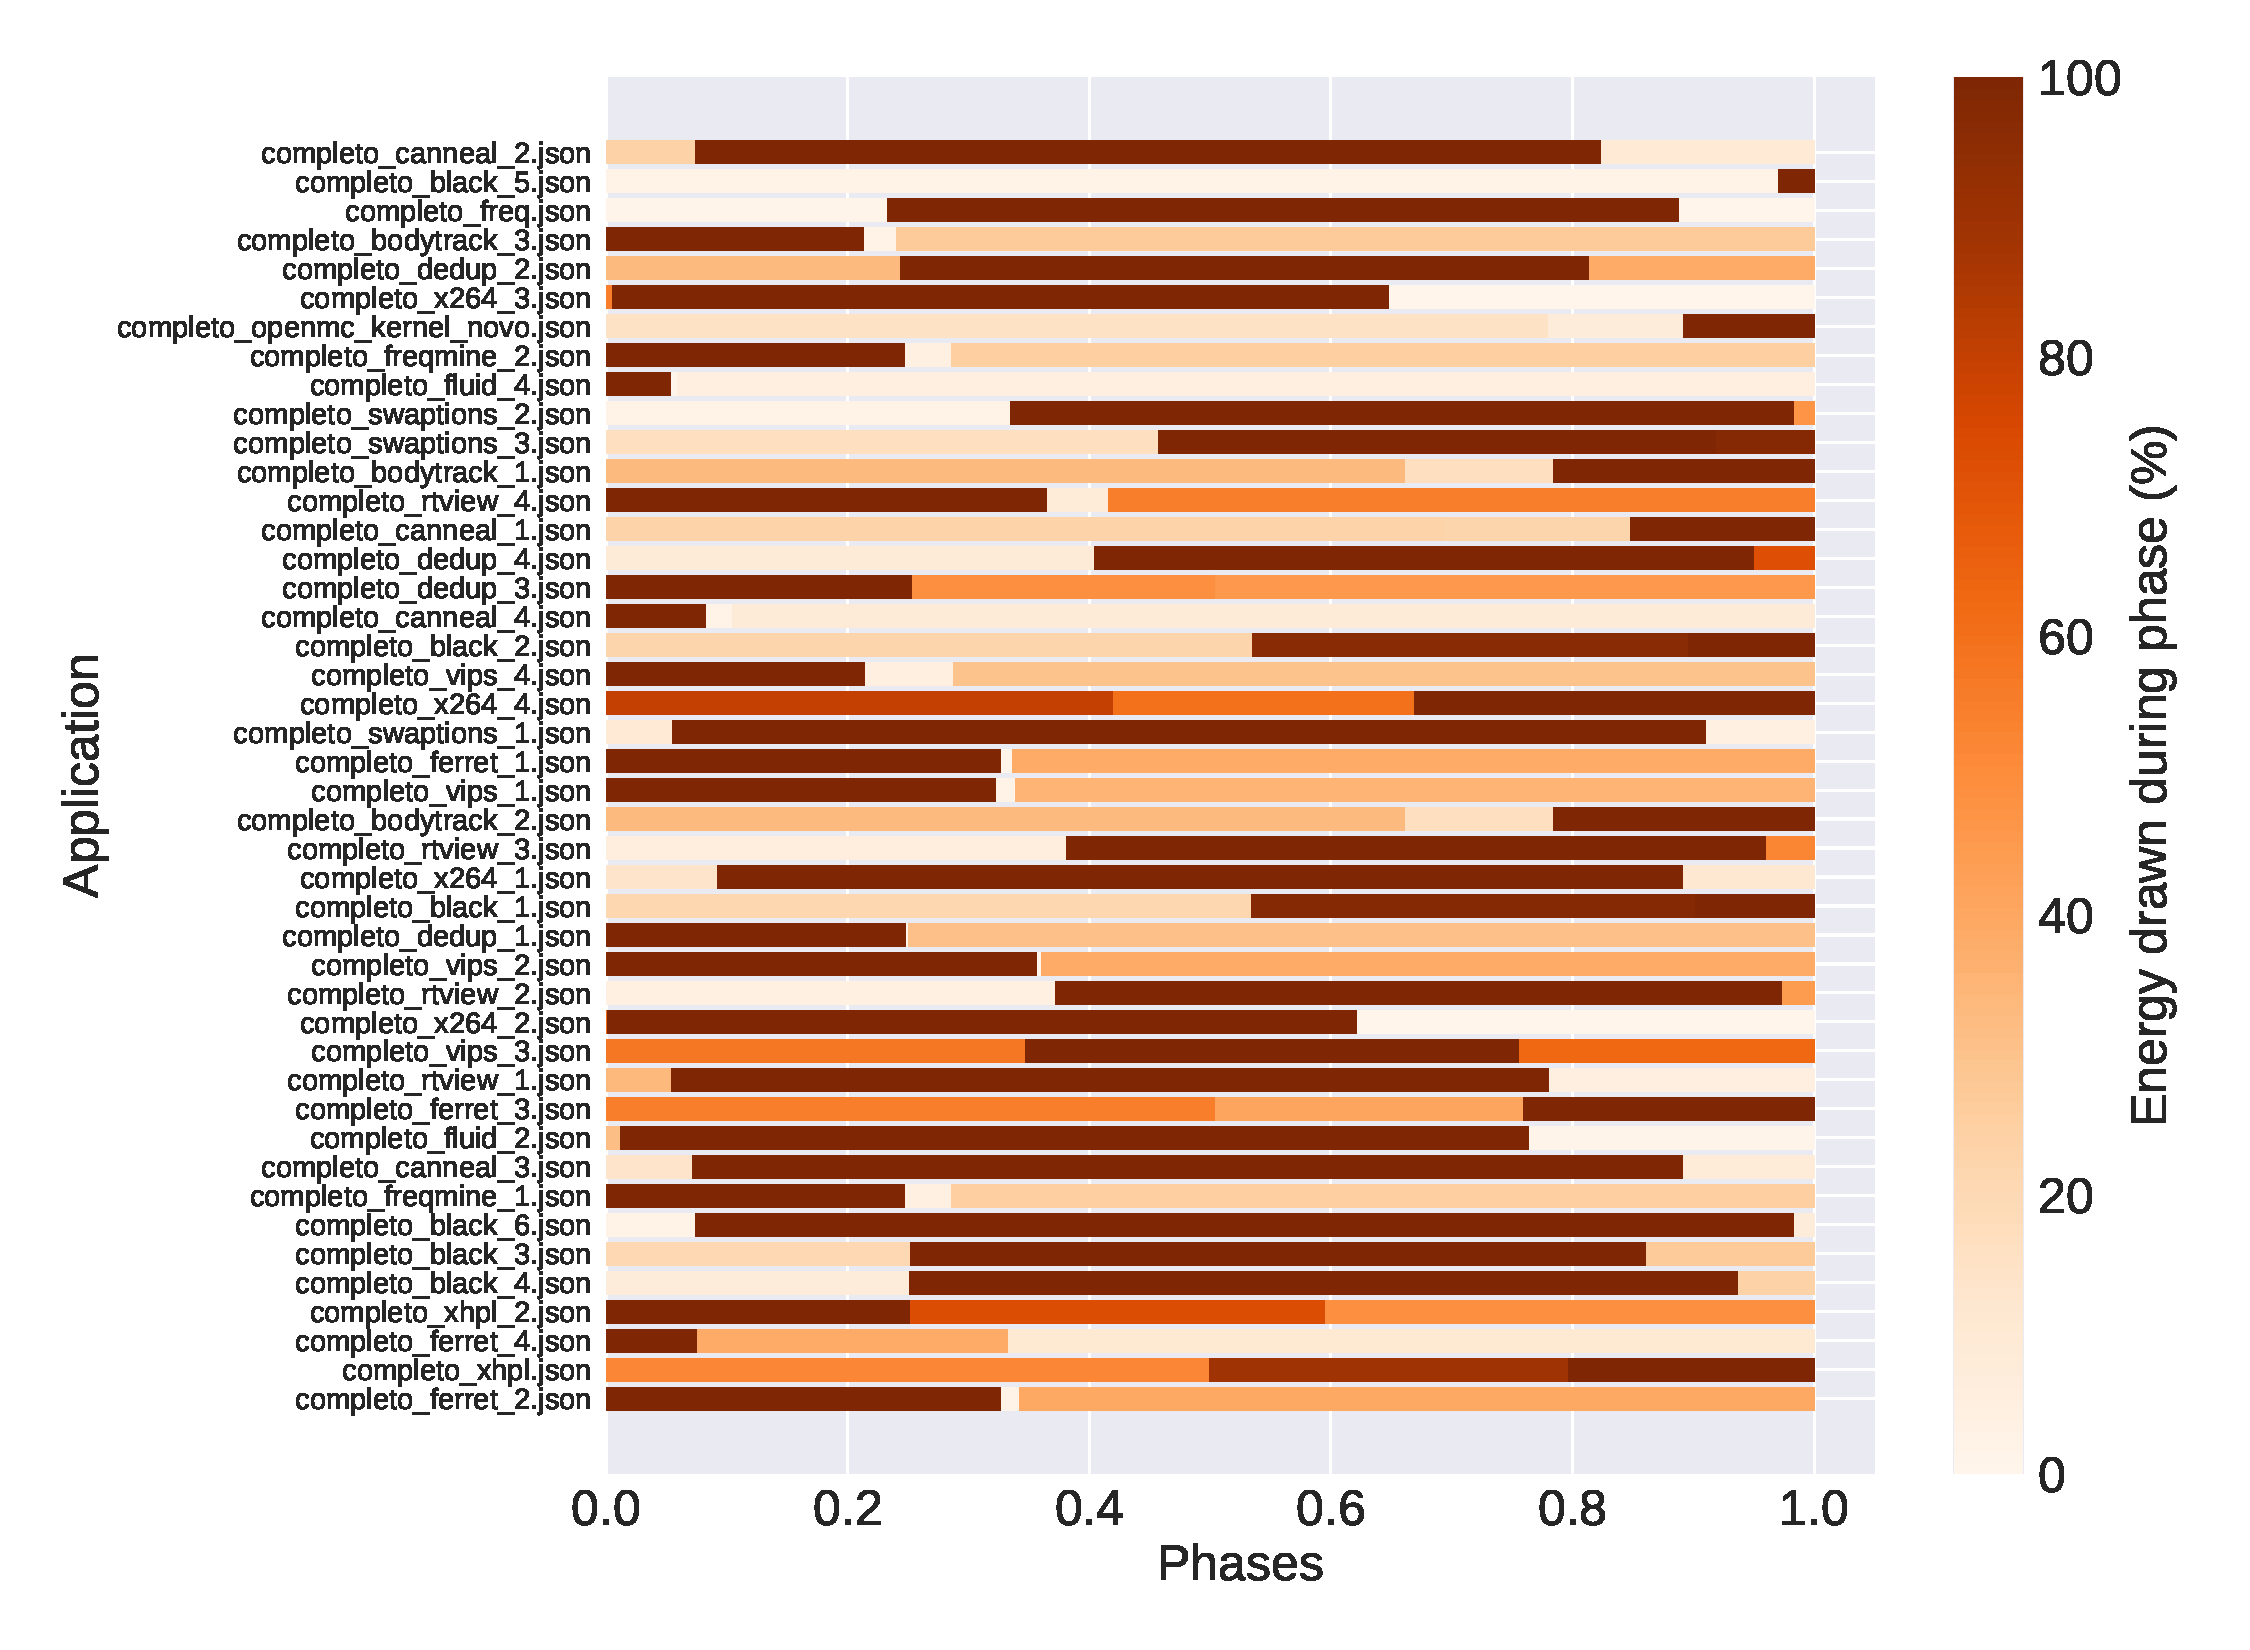
\includegraphics[width=\columnwidth]{phases/figures/phase_division_cmap_3.pdf}
	\caption{Phase division heatmap (3 divisions) showing the energy consumption per phase for all applications.}
	\label{fig:phase_division_cmap_3}
\end{figure}

\begin{figure}[H]
	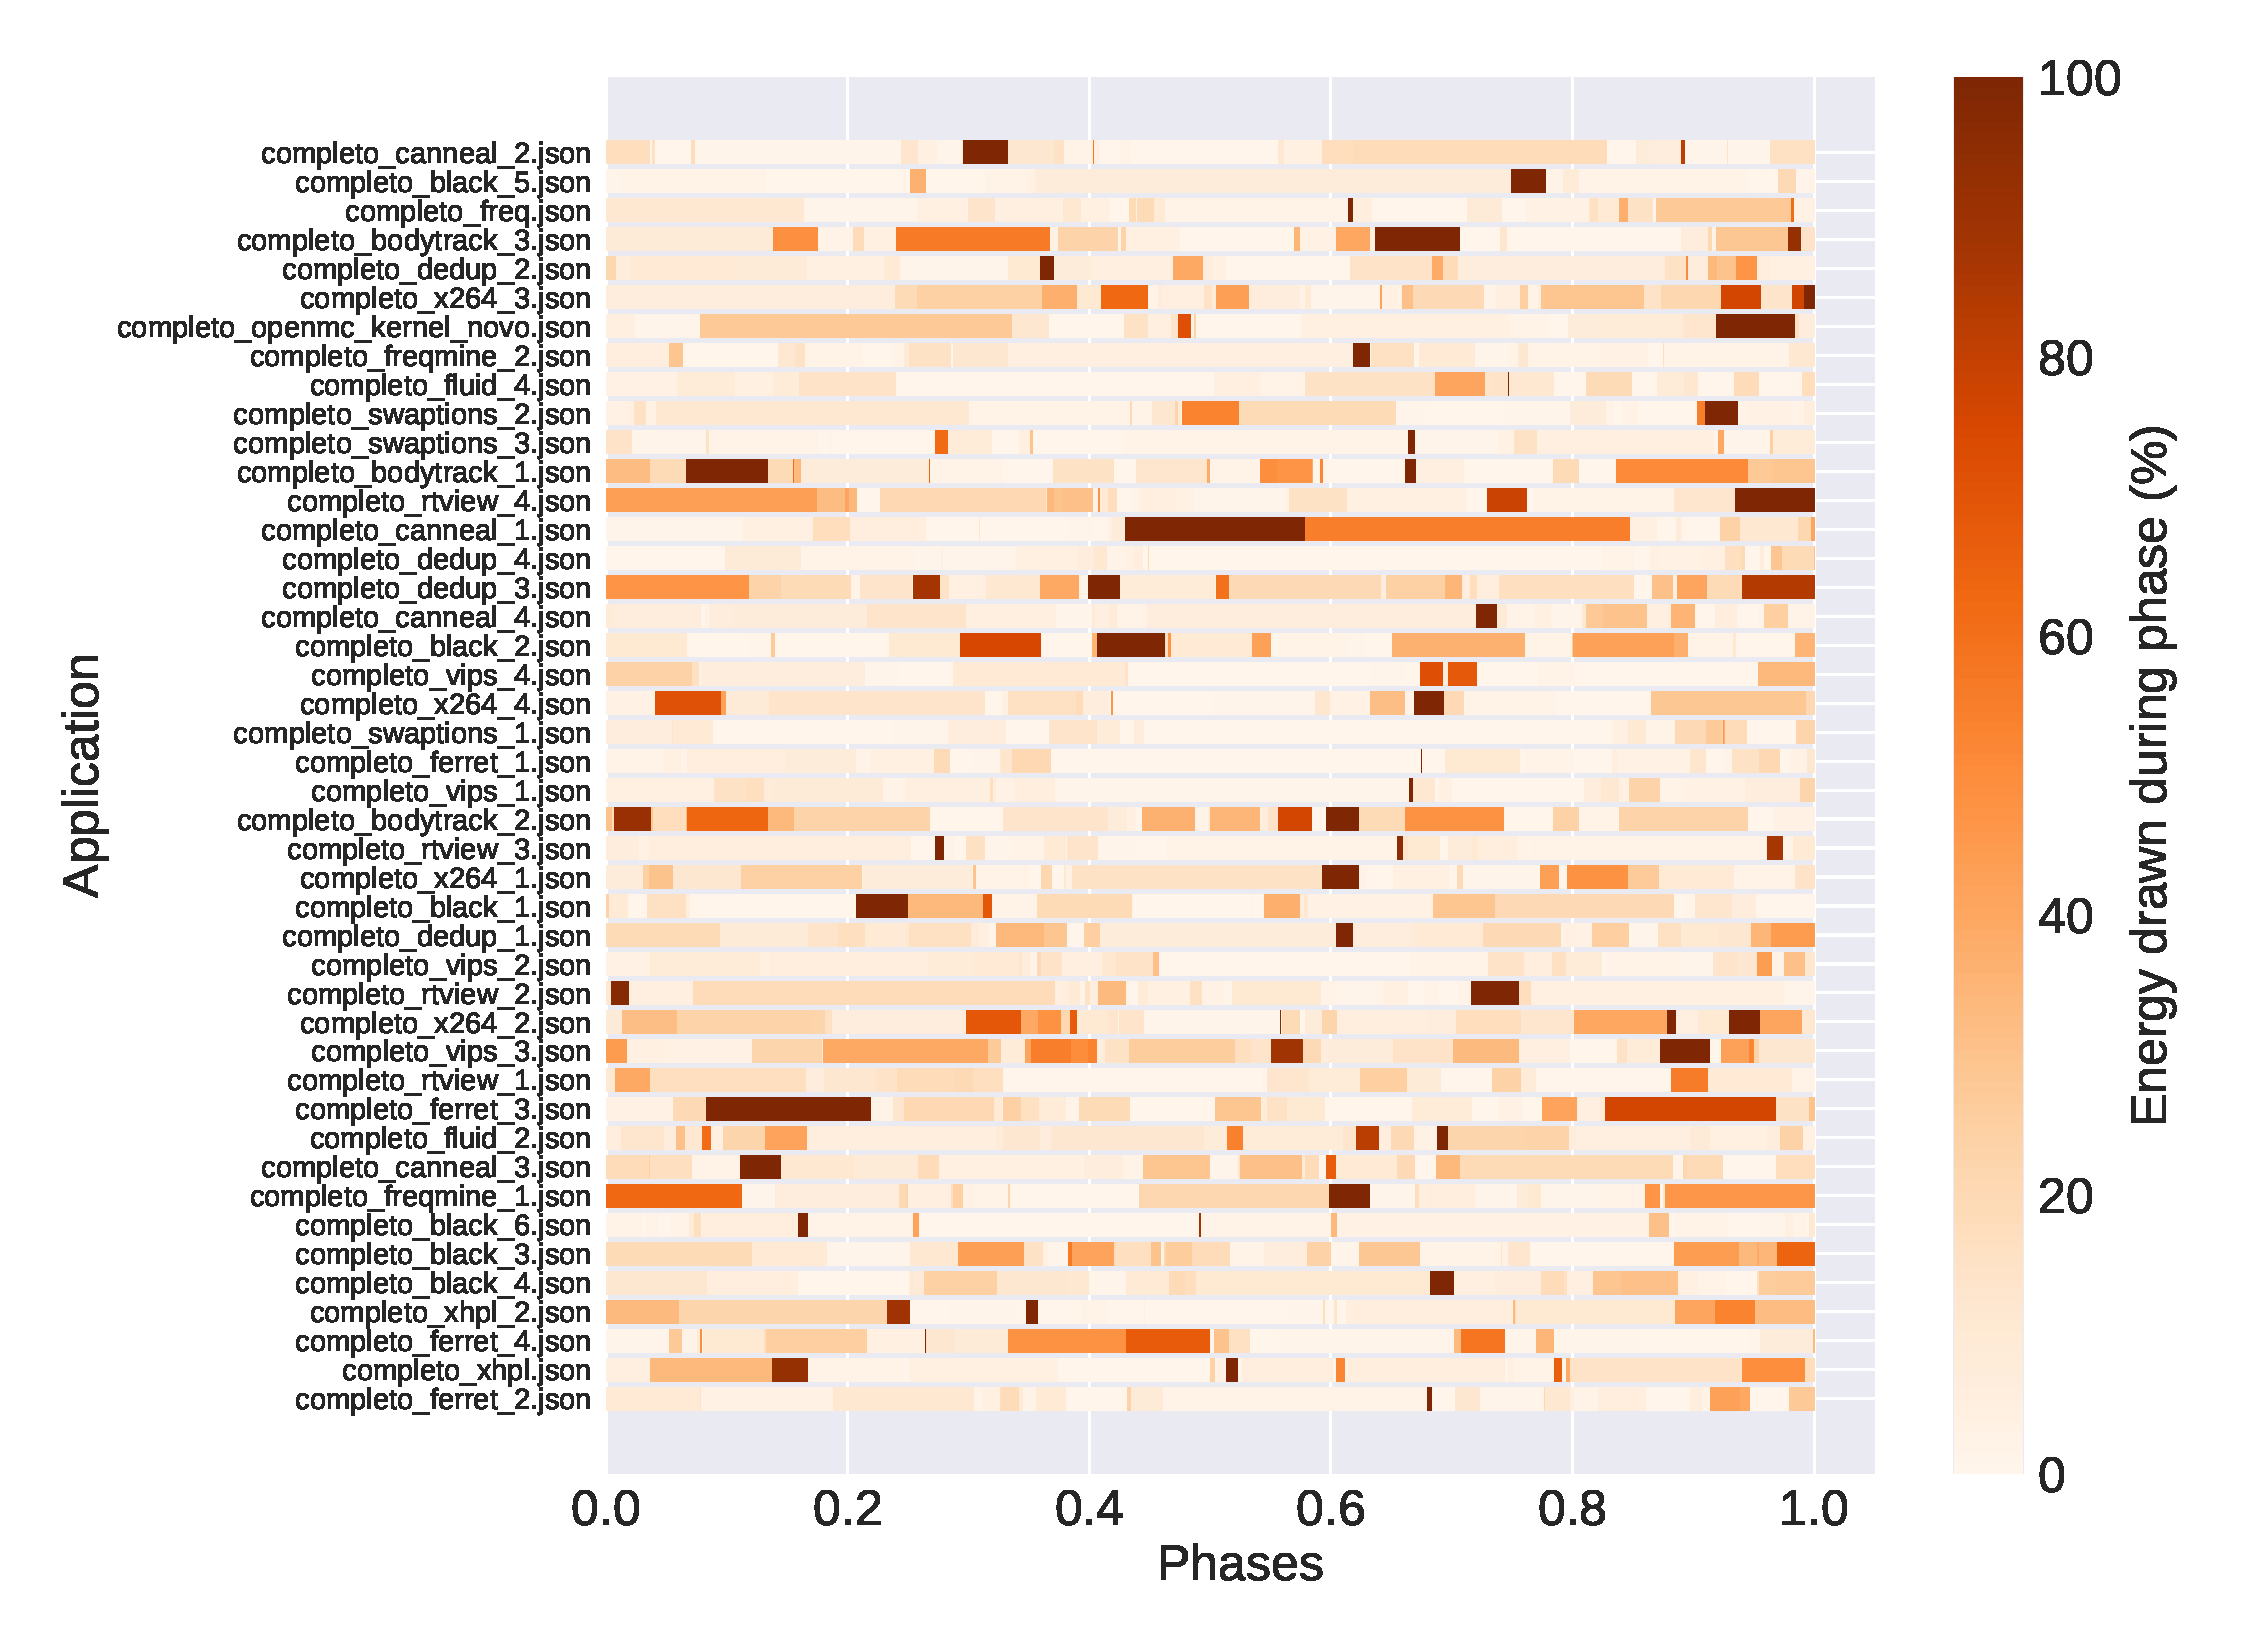
\includegraphics[width=\columnwidth]{phases/figures/phase_division_cmap_35.pdf}
	\caption{Phase division heatmap (35 divisions) showing the energy consumption per phase for all applications.}
	\label{fig:phase_division_cmap_35}
\end{figure}